\documentclass{article}

% Idioma y codificación
\usepackage[spanish, es-tabla]{babel}       %es-tabla para que se titule "Tabla"
\usepackage[utf8]{inputenc}

% Márgenes
\usepackage[a4paper,top=3cm,bottom=2.5cm,left=3cm,right=3cm]{geometry}

% Comentarios de bloque
\usepackage{verbatim}

% Paquetes de links
\usepackage[hidelinks]{hyperref}    % Permite enlaces
\usepackage{url}                    % redirecciona a la web

% Más opciones para enumeraciones
\usepackage{enumitem}

% Personalizar la portada
\usepackage{titling}


% Paquetes de tablas
\usepackage{multirow}


%------------------------------------------------------------------------

%Paquetes de figuras
\usepackage{caption}
\usepackage{subcaption} % Figuras al lado de otras
\usepackage{float}      % Poner figuras en el sitio indicado H.


% Paquetes de imágenes
\usepackage{graphicx}       % Paquete para añadir imágenes
\usepackage{transparent}    % Para manejar la opacidad de las figuras

% Paquete para usar colores
\usepackage[dvipsnames]{xcolor}
\usepackage{pagecolor}      % Para cambiar el color de la página

% Habilita tamaños de fuente mayores
\usepackage{fix-cm}


%------------------------------------------------------------------------

% Paquetes de matemáticas
\usepackage{mathtools, amsfonts, amssymb, mathrsfs}
\usepackage[makeroom]{cancel}     % Simplificar tachando
\usepackage{polynom}    % Divisiones y Ruffini
\usepackage{units} % Para poner fracciones diagonales con \nicefrac

\usepackage{pgfplots}   %Representar funciones
\pgfplotsset{compat=1.18}  % Versión 1.18

\usepackage{tikz-cd}    % Para usar diagramas de composiciones
\usetikzlibrary{calc}   % Para usar cálculo de coordenadas en tikz

%Definición de teoremas, etc.
\usepackage{amsthm}
%\swapnumbers   % Intercambia la posición del texto y de la numeración

\theoremstyle{plain}

\makeatletter
\@ifclassloaded{article}{
  \newtheorem{teo}{Teorema}[section]
}{
  \newtheorem{teo}{Teorema}[chapter]  % Se resetea en cada chapter
}
\makeatother

\newtheorem{coro}{Corolario}[teo]           % Se resetea en cada teorema
\newtheorem{prop}[teo]{Proposición}         % Usa el mismo contador que teorema
\newtheorem{lema}[teo]{Lema}                % Usa el mismo contador que teorema

\theoremstyle{remark}
\newtheorem*{observacion}{Observación}

\theoremstyle{definition}

\makeatletter
\@ifclassloaded{article}{
  \newtheorem{definicion}{Definición} [section]     % Se resetea en cada chapter
}{
  \newtheorem{definicion}{Definición} [chapter]     % Se resetea en cada chapter
}
\makeatother

\newtheorem*{notacion}{Notación}
\newtheorem*{ejemplo}{Ejemplo}
\newtheorem*{ejercicio*}{Ejercicio}             % No numerado
\newtheorem{ejercicio}{Ejercicio} [section]     % Se resetea en cada section


% Modificar el formato de la numeración del teorema "ejercicio"
\renewcommand{\theejercicio}{%
  \ifnum\value{section}=0 % Si no se ha iniciado ninguna sección
    \arabic{ejercicio}% Solo mostrar el número de ejercicio
  \else
    \thesection.\arabic{ejercicio}% Mostrar número de sección y número de ejercicio
  \fi
}


% \renewcommand\qedsymbol{$\blacksquare$}         % Cambiar símbolo QED
%------------------------------------------------------------------------

% Paquetes para encabezados
\usepackage{fancyhdr}
\pagestyle{fancy}
\fancyhf{}

\newcommand{\helv}{ % Modificación tamaño de letra
\fontfamily{}\fontsize{12}{12}\selectfont}
\setlength{\headheight}{15pt} % Amplía el tamaño del índice


%\usepackage{lastpage}   % Referenciar última pag   \pageref{LastPage}
\fancyfoot[C]{\thepage}

%------------------------------------------------------------------------

% Conseguir que no ponga "Capítulo 1". Sino solo "1."
\makeatletter
\@ifclassloaded{book}{
  \renewcommand{\chaptermark}[1]{\markboth{\thechapter.\ #1}{}} % En el encabezado
    
  \renewcommand{\@makechapterhead}[1]{%
  \vspace*{50\p@}%
  {\parindent \z@ \raggedright \normalfont
    \ifnum \c@secnumdepth >\m@ne
      \huge\bfseries \thechapter.\hspace{1em}\ignorespaces
    \fi
    \interlinepenalty\@M
    \Huge \bfseries #1\par\nobreak
    \vskip 40\p@
  }}
}
\makeatother

%------------------------------------------------------------------------
% Paquetes de cógido
\usepackage{minted}
\renewcommand\listingscaption{Código fuente}

\usepackage{fancyvrb}
% Personaliza el tamaño de los números de línea
\renewcommand{\theFancyVerbLine}{\small\arabic{FancyVerbLine}}

% Estilo para C++
\newminted{cpp}{
    frame=lines,
    framesep=2mm,
    baselinestretch=1.2,
    linenos,
    escapeinside=||
}



\usepackage{listings} % Para incluir código desde un archivo

\renewcommand\lstlistingname{Código Fuente}
\renewcommand\lstlistlistingname{Índice de Códigos Fuente}

% Definir colores
\definecolor{vscodepurple}{rgb}{0.5,0,0.5}
\definecolor{vscodeblue}{rgb}{0,0,0.8}
\definecolor{vscodegreen}{rgb}{0,0.5,0}
\definecolor{vscodegray}{rgb}{0.5,0.5,0.5}
\definecolor{vscodebackground}{rgb}{0.97,0.97,0.97}
\definecolor{vscodelightgray}{rgb}{0.9,0.9,0.9}

% Configuración para el estilo de C similar a VSCode
\lstdefinestyle{vscode_C}{
  backgroundcolor=\color{vscodebackground},
  commentstyle=\color{vscodegreen},
  keywordstyle=\color{vscodeblue},
  numberstyle=\tiny\color{vscodegray},
  stringstyle=\color{vscodepurple},
  basicstyle=\scriptsize\ttfamily,
  breakatwhitespace=false,
  breaklines=true,
  captionpos=b,
  keepspaces=true,
  numbers=left,
  numbersep=5pt,
  showspaces=false,
  showstringspaces=false,
  showtabs=false,
  tabsize=2,
  frame=tb,
  framerule=0pt,
  aboveskip=10pt,
  belowskip=10pt,
  xleftmargin=10pt,
  xrightmargin=10pt,
  framexleftmargin=10pt,
  framexrightmargin=10pt,
  framesep=0pt,
  rulecolor=\color{vscodelightgray},
  backgroundcolor=\color{vscodebackground},
}

%------------------------------------------------------------------------

% Comandos definidos
\newcommand{\bb}[1]{\mathbb{#1}}
\newcommand{\cc}[1]{\mathcal{#1}}

% I prefer the slanted \leq
\let\oldleq\leq % save them in case they're every wanted
\let\oldgeq\geq
\renewcommand{\leq}{\leqslant}
\renewcommand{\geq}{\geqslant}

% Si y solo si
\newcommand{\sii}{\iff}

% Letras griegas
\newcommand{\eps}{\epsilon}
\newcommand{\veps}{\varepsilon}
\newcommand{\lm}{\lambda}

\newcommand{\ol}{\overline}
\newcommand{\ul}{\underline}
\newcommand{\wt}{\widetilde}
\newcommand{\wh}{\widehat}

\let\oldvec\vec
\renewcommand{\vec}{\overrightarrow}

% Derivadas parciales
\newcommand{\del}[2]{\frac{\partial #1}{\partial #2}}
\newcommand{\Del}[3]{\frac{\partial^{#1} #2}{\partial^{#1} #3}}
\newcommand{\deld}[2]{\dfrac{\partial #1}{\partial #2}}
\newcommand{\Deld}[3]{\dfrac{\partial^{#1} #2}{\partial^{#1} #3}}


\newcommand{\AstIg}{\stackrel{(\ast)}{=}}
\newcommand{\Hop}{\stackrel{L'H\hat{o}pital}{=}}

\newcommand{\red}[1]{{\color{red}#1}} % Para integrales, destacar los cambios.

% Método de integración
\newcommand{\MetInt}[2]{
    \left[\begin{array}{c}
        #1 \\ #2
    \end{array}\right]
}

% Declarar aplicaciones
% 1. Nombre aplicación
% 2. Dominio
% 3. Codominio
% 4. Variable
% 5. Imagen de la variable
\newcommand{\Func}[5]{
    \begin{equation*}
        \begin{array}{rrll}
            #1:& #2 & \longrightarrow & #3\\
               & #4 & \longmapsto & #5
        \end{array}
    \end{equation*}
}

%------------------------------------------------------------------------

% Define a custom command for email addresses
\newcommand{\email}[1]{\href{mailto:#1}{{{\color{blue}#1}}}}


\usepackage{schemata}
\usepackage{ragged2e}
\usepackage{booktabs}
\lstset{
    literate={á}{{\'a}}1
             {é}{{\'e}}1
             {ó}{{\'o}}1
             {í}{{\'i}}1
             {ú}{{\'u}}1
             % Agrega más caracteres si es necesario
}

\definecolor{codegreen}{rgb}{0,0.6,0}
\definecolor{codegray}{rgb}{0.5,0.5,0.5}
\definecolor{codepurple}{rgb}{0.58,0,0.82}
\definecolor{backcolour}{rgb}{0.95,0.95,0.92}

\definecolor{backcolor}{RGB}{30,30,30}
\definecolor{codeblue}{RGB}{153,255,255}
\definecolor{codepink}{RGB}{200,80,180}
\definecolor{normalblue}{RGB}{12,144,244}

\lstdefinestyle{vscodestyle0}{
    backgroundcolor=\color{backcolor},   
    commentstyle=\color{codegreen},
    keywordstyle=\color{codepink},
    numberstyle=\tiny\color{codegray},
    identifierstyle=\color{codeblue},
    rulecolor=\color{black},
    stringstyle=\color{codepurple},
    basicstyle=\ttfamily\footnotesize,
    breakatwhitespace=false,         
    breaklines=true,                 
    captionpos=b,                    
    keepspaces=true,                 
    numbers=left,                    
    numbersep=5pt,                  
    showspaces=false,                
    showstringspaces=false,
    showtabs=false,                  
    tabsize=2,
    literate=%
  {\ +\ }{{{\color{Red}\ +\ }}}1
  {\ -\ }{{{\color{Red}\ -\ }}}1
  {\ *\ }{{{\color{Red}\ *\ }}}1
  {\ /\ }{{{\color{Red}\ /\ }}}1
  {\ =\ }{{{\color{Red}\ =\ }}}1
}

\lstdefinestyle{vscodestyle}{
    backgroundcolor=\color{backcolor},    % Fondo oscuro
    basicstyle=\color{white}\ttfamily\footnotesize, % Texto en blanco
    commentstyle=\color{green!50!black}, % Estilo de comentarios
    keywordstyle=\color{codepink},       % Estilo de palabras clave
    keywordstyle={[2]\color{blue}}, % Estilo para tipos de datos (int, char, double, etc.)
    identifierstyle=\color{codeblue},
    numberstyle=\tiny\color{gray},   % Estilo de números de línea
    stringstyle=\color{orange},      % Estilo de cadenas de texto
    rulecolor=\color{black},
    breakatwhitespace=false,         % Romper líneas solo en espacios en blanco
    breaklines=true,                 % Romper líneas automáticamente
    captionpos=b,                    % Posición de la leyenda (abajo)
    keepspaces=true,                 % Conservar espacios en blanco
    numbers=left,                    % Mostrar números de línea a la izquierda
    numbersep=5pt,                   % Separación de números de línea del código
    showspaces=false,                % Mostrar espacios con guiones bajos
    showstringspaces=false,          % No subrayar espacios en cadenas de texto
    showtabs=false,                  % No mostrar tabulaciones
    tabsize=4                        % Tamaño de la tabulación
}

\lstset{
    language=C++,
    morekeywords={int,char,ld,double}
}


\lstdefinestyle{mystyle}{
    backgroundcolor=\color{backcolour},   
    commentstyle=\color{codegreen},
    keywordstyle=\color{magenta},
    numberstyle=\tiny\color{codegray},
    stringstyle=\color{codepurple},
    %identifierstyle=\color{blue},
    basicstyle=\ttfamily\footnotesize,
    breakatwhitespace=false,         
    breaklines=true,                 
    captionpos=b,                    
    keepspaces=true,                 
    numbers=left,                    
    numbersep=5pt,                  
    showspaces=false,                
    showstringspaces=false,
    showtabs=false,                  
    tabsize=2
}
%\usemintedstyle[C++]{default}
\lstset{style=mystyle}

\newcommand{\myparagraph}[1]{\paragraph{#1}\mbox{}\\}
\newcommand\N{\ensuremath{\mathbb N}\space} 



\hypersetup{
    colorlinks=false, % Establece 'true' si quieres que el texto del enlace sea de color en lugar de tener un cuadro
    pdfborder={0 0 0}, % Establece el borde del enlace a 0 para eliminarlo
}



\begin{document}

    % 1. Foto de fondo
    % 2. Título
    % 3. Encabezado Izquierdo
    % 4. Color de fondo
    % 5. Coord x del titulo
    % 6. Coord y del titulo
    % 7. Fecha
    % 8. Autor

    
    % 1. Foto de fondo
% 2. Título
% 3. Encabezado Izquierdo
% 4. Color de fondo
% 5. Coord x del titulo
% 6. Coord y del titulo
% 7. Fecha

\newcommand{\portada}[7]{

    \portadaBase{#1}{#2}{#3}{#4}{#5}{#6}{#7}
    \portadaBook{#1}{#2}{#3}{#4}{#5}{#6}{#7}
}

\newcommand{\portadaExamen}[7]{

    \portadaBase{#1}{#2}{#3}{#4}{#5}{#6}{#7}
    \portadaArticle{#1}{#2}{#3}{#4}{#5}{#6}{#7}
}




\newcommand{\portadaBase}[7]{

    % Tiene la portada principal y la licencia Creative Commons
    
    % 1. Foto de fondo
    % 2. Título
    % 3. Encabezado Izquierdo
    % 4. Color de fondo
    % 5. Coord x del titulo
    % 6. Coord y del titulo
    % 7. Fecha
    
    
    \thispagestyle{empty}               % Sin encabezado ni pie de página
    \newgeometry{margin=0cm}        % Márgenes nulos para la primera página
    
    
    % Encabezado
    \fancyhead[L]{\helv #3}
    \fancyhead[R]{\helv \nouppercase{\leftmark}}
    
    
    \pagecolor{#4}        % Color de fondo para la portada
    
    \begin{figure}[p]
        \centering
        \transparent{0.3}           % Opacidad del 30% para la imagen
        
        \includegraphics[width=\paperwidth, keepaspectratio]{assets/#1}
    
        \begin{tikzpicture}[remember picture, overlay]
            \node[anchor=north west, text=white, opacity=1, font=\fontsize{60}{90}\selectfont\bfseries\sffamily, align=left] at (#5, #6) {#2};
            
            \node[anchor=south east, text=white, opacity=1, font=\fontsize{12}{18}\selectfont\sffamily, align=right] at (9.7, 3) {\textbf{\href{https://losdeldgiim.github.io/}{Los Del DGIIM}}};
            
            \node[anchor=south east, text=white, opacity=1, font=\fontsize{12}{15}\selectfont\sffamily, align=right] at (9.7, 1.8) {Doble Grado en Ingeniería Informática y Matemáticas\\Universidad de Granada};
        \end{tikzpicture}
    \end{figure}
    
    
    \restoregeometry        % Restaurar márgenes normales para las páginas subsiguientes
    \pagecolor{white}       % Restaurar el color de página
    
    
    \newpage
    \thispagestyle{empty}               % Sin encabezado ni pie de página
    \begin{tikzpicture}[remember picture, overlay]
        \node[anchor=south west, inner sep=3cm] at (current page.south west) {
            \begin{minipage}{0.5\paperwidth}
                \href{https://creativecommons.org/licenses/by-nc-nd/4.0/}{
                    
\includegraphics[height=2cm]{assets/Licencia.png}
                }\vspace{1cm}\\
                Esta obra está bajo una
                \href{https://creativecommons.org/licenses/by-nc-nd/4.0/}{
                    Licencia Creative Commons Atribución-NoComercial-SinDerivadas 4.0 Internacional (CC BY-NC-ND 4.0).
                }\\
    
                Eres libre de compartir y redistribuir el contenido de esta obra en cualquier medio o formato, siempre y cuando des el crédito adecuado a los autores originales y no persigas fines comerciales. 
            \end{minipage}
        };
    \end{tikzpicture}
    
    
    
    % 1. Foto de fondo
    % 2. Título
    % 3. Encabezado Izquierdo
    % 4. Color de fondo
    % 5. Coord x del titulo
    % 6. Coord y del titulo
    % 7. Fecha


}


\newcommand{\portadaBook}[7]{

    % 1. Foto de fondo
    % 2. Título
    % 3. Encabezado Izquierdo
    % 4. Color de fondo
    % 5. Coord x del titulo
    % 6. Coord y del titulo
    % 7. Fecha

    % Personaliza el formato del título
    \pretitle{\begin{center}\bfseries\fontsize{42}{56}\selectfont}
    \posttitle{\par\end{center}\vspace{2em}}
    
    % Personaliza el formato del autor
    \preauthor{\begin{center}\Large}
    \postauthor{\par\end{center}\vfill}
    
    % Personaliza el formato de la fecha
    \predate{\begin{center}\huge}
    \postdate{\par\end{center}\vspace{2em}}
    
    \title{#2}
    \author{\href{https://losdeldgiim.github.io/}{Los Del DGIIM}}
    \date{Granada, #7}
    \maketitle
    
    \tableofcontents
}




\newcommand{\portadaArticle}[7]{

    % 1. Foto de fondo
    % 2. Título
    % 3. Encabezado Izquierdo
    % 4. Color de fondo
    % 5. Coord x del titulo
    % 6. Coord y del titulo
    % 7. Fecha

    % Personaliza el formato del título
    \pretitle{\begin{center}\bfseries\fontsize{42}{56}\selectfont}
    \posttitle{\par\end{center}\vspace{2em}}
    
    % Personaliza el formato del autor
    \preauthor{\begin{center}\Large}
    \postauthor{\par\end{center}\vspace{3em}}
    
    % Personaliza el formato de la fecha
    \predate{\begin{center}\huge}
    \postdate{\par\end{center}\vspace{5em}}
    
    \title{#2}
    \author{\href{https://losdeldgiim.github.io/}{Los Del DGIIM}}
    \date{Granada, #7}
    \thispagestyle{empty}               % Sin encabezado ni pie de página
    \maketitle
    \vfill
}
    \portada{etsiitA4.jpg}{Algorítmica\\Práctica 3}{Algorítmica. Práctica 3. Greedy.}{MidnightBlue}{-8}{28}{2023-2024}{Laura Mandow Fuentes\\Chengcheng Liu\\Daniel Hidalgo Chica\\Roberto González Lugo\\Elías Monge Sánchez}

    \newpage

    
\section{Participación}
    \begin{itemize}
        \item Laura Mandow Fuentes. \email{e.lauramandow@go.ugr.es}  $100\%$
        \item Roberto González Lugo. \email{e.roberlks222@go.ugr.es}  $100\%$
        \item Daniel Hidalgo Chica. \email{e.danielhc@go.ugr.es}  $100\%$
        \item Chengcheng Liu. \email{e.cliu04@go.ugr.es} $100\%$
        \item Elías Monge Sánchez. \email{e.eliasmonge234@go.ugr.es}  $100\%$
    \end{itemize}
    \subsection{Participación específica}
    Aunque hayamos trabajado cada uno de forma global los contenidos de la práctica, a la hora de la redacción de la memoria, el trabajo se ha visto dividido en partes de carga de trabajo similar con el fin de aumentar la productividad.
    \\
    En particular, las máquinas utilizadas para ejecutar los algoritmos son:
    \begin{itemize}
        \item P1
        \begin{itemize}
                \item Máquina: Asus TUF fx505dt
                \item Procesador: AMD Ryzen 7 3750h with Radeon Vega Mobile Gfx 2.3GHz
                \item Tarjeta gráfica: Nvidia Geforce GTX 1650
                \item Sistema Operativo: Arch Linux 64bits
        \end{itemize}

        \item P2
        \begin{itemize}

                \item Máquina: Acer Aspire A315-42
                \item Procesador: Procesador: AMD Ryzen 5 3500U 2.10 GHz
                \item Tarjeta Gráfica: Radeon Vega Mobile Gfx
                \item Sistema Operativo: Ubuntu 22.04 64bits (Oracle VM VirtualBox, 2 cores)
                        \end{itemize}

        \item P3
            \begin{itemize}
                \item Máquina: HP Laptop 15s-eq1xxx
                \item Procesador:AMD Ryzen 5 4500U with Radeon Graphics
                \item Sistema Operativo: Ubuntu 22.04 64 bits
            \end{itemize}
        \item P4
        \begin{itemize}
            \item V1        \begin{itemize}
                \item Máquina: HP Laptop 15s-eq1xxx
                \item Procesador:AMD Ryzen 5 4500U with Radeon Graphics
                \item Sistema Operativo: Ubuntu 22.04 64 bits
            \end{itemize}
            \item V2        \begin{itemize}
                \item Máquina: Surface Laptop 4
                \item Procesador: Intel Core i7
                \item Tarjeta Gráfica: Intel Corporation TigerLake-LP GT2 [Iris Xe Graphics] (rev 01)
                \item Sistema Operativo: Ubuntu 22.04 64bits
            \end{itemize}
            \item V3        \begin{itemize}
                \item Máquina: HP Laptop 15s-eq1xxx
                \item Procesador:AMD Ryzen 5 4500U with Radeon Graphics
                \item Sistema Operativo: Ubuntu 22.04 64 bits
            \end{itemize}
        \end{itemize}
        


    \end{itemize}
        
\newpage
\section{Objetivos}
Los objetivos de esta práctica se enfocan en la \textbf{comprensión y asimilación profunda} de la técnica de diseño de algoritmos voraces (\textit{greedy algorithms}), aplicada a la resolución de problemas complejos mediante un enfoque sistemático y estratégico. Esta técnica se caracteriza por tomar decisiones secuenciales que parecen óptimas en el momento, con el fin de alcanzar una solución global eficiente. A través de esta metodología, los estudiantes aprenderán a descomponer los problemas y aplicar la estrategia voraz para lograr soluciones exactas o aproximadas.


Además, se promoverá el desarrollo de \textbf{heurísticas y algoritmos aproximativos} basados en la filosofía de los métodos voraces, especialmente útiles en situaciones donde no se conocen soluciones eficientes. Esta práctica, realizada en grupos, también fomentará habilidades de trabajo colaborativo y de comunicación efectiva, permitiendo el intercambio de ideas y la adaptación de las soluciones a diferentes contextos y tipos de problemas.

Por lo tanto, nuestros objetivos no solo incluyen el diseño e implementación de algoritmos siguiendo las directrices específicas, sino también una \textbf{profunda comprensión teórica} de los principios subyacentes a los algoritmos voraces. Buscamos desarrollar competencias técnicas en la solución de problemas y habilidades transversales que potencien la formación académica y profesional de los estudiantes en la ciencia de la computación.

En conclusión, los objetivos de nuestra práctica abarcan el \textbf{dominio de la técnica de algoritmos voraces} para el diseño y desarrollo de soluciones a problemas complejos, la capacidad para implementar soluciones efectivas y la habilidad para trabajar en equipo y comunicarse de manera efectiva, todo dentro de un marco que complementa y enriquece su formación técnica en la disciplina.



\newpage

\section{P1 Problema del hijo predilecto}
\subsection{Diseño del algoritmo}
\subsubsection{Descripción del problema}
Un individuo desea repartir sus $N$ bienes entre sus 2 hijos. Para cada bien se conoce el valor (positivo) del mismo. Previo al fallecimiento del individuo, el juzgado, de una forma ciega, determina un valor k, que nos indica el número de bienes que se le deben asignar a un hijo (al otro se le asignan $N$ - $k$). Conocido estos datos, el individuo desea distribuir los bienes entre sus hijos de forma que uno de ellos salga lo mas beneficiado posible. El beneficio obtenido por cada hijo se define como la suma de los beneficios de los bienes que se les lega.
\subsubsection{Algoritmo Greedy}
Proponemos una solución al problema que consiste en, una vez ordenados los bienes según su valor (de menor a mayor), se elije si el hijo predilecto tendrá $k$ o $N-k$ bienes ¿$(k\leq \frac N2)$?, y en función de eso se rellenan los vectores del hijo predilecto y del otro, primero el del otro hijo, y después el del predilecto. Esto es debido a que los bienes están ordenados de menor a mayor (en un set)
\subsubsection{Componentes y demostración de validez}


Las componentes del algoritmo greedy son:

\begin{itemize}
    \item \textbf{Previo:} De aquí en adelante, si $k\leq  \frac{N}{2}$, el hijo predilecto recibirá $N-k$ bienes, sino, recibirá $k$ bienes. A este tamaño, lo llamaremos $tam$
    \item \textbf{Conjunto candidatos:} Los diferentes valores de los bienes del problema
    \item \textbf{Conjunto seleccionados:} Los $tam$ bienes del hijo predilecto
     \item \textbf{Función selección:} En cada paso, se añade el bien con mayor valor
\end{itemize}
A continuación, demostraremos la validez del algoritmo Greedy por inducción:
\begin{itemize}
    \item \textbf{Caso base:} (Red abs) Consideramos que tenemos un conjunto solución $B$ que no incluye al bien con valor máximo (Sea $B_m$). El valor total de los bienes será $V(B)$ Introducimos $B_m$ en la solución, y quitamos cualquier otro elemento $b_n$, entonces, el valor de este nuevo conjunto es $V(B) + V(B_m) - V(b_n)$, pero como $V(B_m) > V(b_n) \implies V(B)+ V(B_m) - V(b_n)  > V(B)$ CONTRADICCIÓN
    \item \textbf{Paso de inducción:} 
    Consideramos un conjunto solución $B'$ que incluye a $\{b_1,...b_{m-1}\}$ y no incluye a $b_m$ (Siendo $V(b_m) > V(b_n)$ para algún $n\in \{1,...(m-1)\}$, entonces, introduciendo $b_m$ en el conjunto y eliminando $b_n$, tenemos $V(B') + V(b_m) - v(b_n)$, y como $V(b_m) > V(b_n) \implies V(B') + V(b_m) - v(b_n) > V(B') $ CONTRADICCIÓN.
\end{itemize}
    Queda así demostrada la validez de nuestro algoritmo.
\begin{itemize}
    \item \textbf{NOTA:} Nuestro algoritmo rellena primero el hijo NO predilecto, debido a que hemos elegido ordenar el set por defecto (de menor a mayor), esto no afecta a nuestra demostración, pues es equivalente a ordenarlo de mayor a menor y rellenar primero el hijo predilecto, es una mera cuestión de estilo en el código.
\end{itemize}

\subsection{Implementación y estudio de eficiencias}
\subsubsection{Datos de entrada}
El formato de los datos de entrada para este problema será simple. En primer lugar, recibe la cantidad de bienes con los que se va a trabajar, es decir, nuestra $N$. En segundo lugar (en la siguiente linea), recibe el valor de la $k$, es decir, la cantidad de bienes que tendrá un hijo. Por último (en la siguiente linea), recibe, separados por espacios, el valor de todos los $N$ bienes con los que trabajará. Aquí un ejemplo de entrada para este algoritmo: \newline

$$\begin{matrix}
    10 \\ 5 \\ 61 & 24 & 21 & 81 & 32 & 39 & 24 & 55 & 89 & 30
\end{matrix}$$

\subsubsection{Implementación del algoritmo}
A continuación mostramos la implementación del algoritmo desarrollado, es bastante directa de comprender debido a que se trata de un problema relativamente sencillo.
\begin{itemize}
    \item Primeramente, se comprueban los argumentos y se abren los archivos, se prepara todo para poder leer los datos directamente en orden (añaadiendolos a un set)
 \lstinputlisting[language=C++, firstline=20, lastline = 37]{Problema1/codigos/predilectedSon.cpp}
\item A continuación, la lectura de datos y el algoritmo en sí
\lstinputlisting[language=C++, firstline=38,lastline=71]{Problema1/codigos/predilectedSon.cpp}

\item Teniendo esto, el problema queda resuelto, el resto del código es simplemente contar el tiempo que se ha tardado e imprimir los resultados
\lstinputlisting[language=C++, firstline=72,lastline=94]{Problema1/codigos/predilectedSon.cpp}


\end{itemize}
\subsubsection{Estudio de eficiencia}

\myparagraph{Eficiencia teórica}
    Estudiemos la eficiencia teórica. En primer lugar, el insertado en un set (que incluye la ordenación) es de orden $O(\log (n))$. Como esto se realiza $n$ veces, nos queda, por ahora, $O (n \log (n))$. \newline
    A continuación entramos en el primer $if$, la condición es $O(1)$ así que podemos ignorarla. Distingamos casos: \begin{itemize}
        \item Si entra al $if$: El $for$ se ejecutará $k$ veces, haciendo una inserción en un vector, y un borrado del set, lo cual es $O(1)$ y $O(\log (n))$ respectivamente. Por ahora, dentro de este if, tendremos un $O(k \log (n))$
        A continuación entra en el $while$, donde ejecutará $N-k$ veces, y por cada iteración le cuesta lo mismo que al if, así que en total tenemos $O(k \log (n)) + O((N-k) \log (n)) = O(n \log (n))$
        \item Si no entra al $if$: realmente pasará lo mismo que si hubiera entrado, ya que el código es el mismo pero en el orden contrario, quedando así $O((N-k) \log (n)) + O(k \log (n)) = O(n \log (n))$
    \end{itemize}
    Si juntamos esto con el $O(n \log (n))$ que teníamos ya, nos queda: $O(n \log (n) + n \log (n)) = O (2n \log (n)) = O(n \log (n))$
\myparagraph{Eficiencia empírica e híbrida}
En cuanto a la eficiencia empírica, ejecutando casos desde $200000$ y hasta $900000$ con saltos de $20000$, nos queda la siguiente gráfica de tiempos:
   \begin{figure}[H]
    \begin{subfigure}{0.4\textwidth}
        \centering
        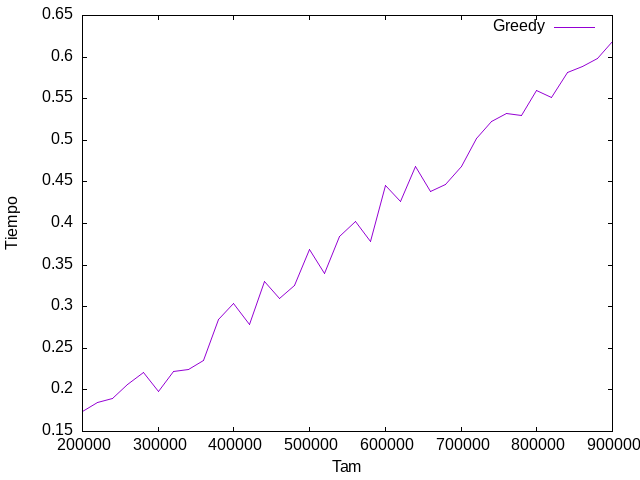
\includegraphics[scale = 0.40]{Problema1/Imagenes/GraficaLineas.jpeg}
    \end{subfigure} \hfill
    \begin{subfigure}{0.4\textwidth}
        \centering
        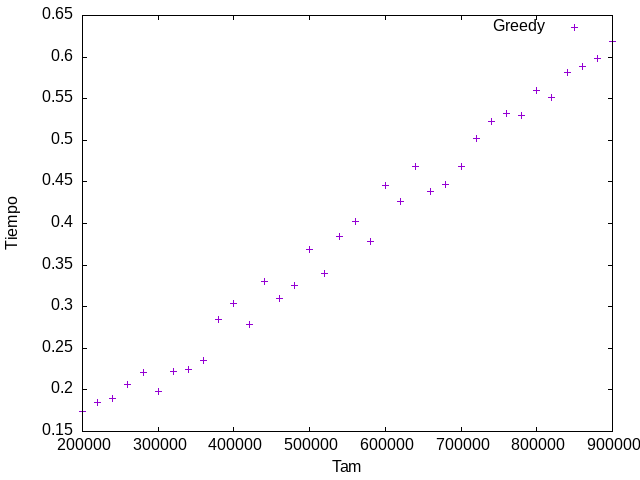
\includegraphics[scale = 0.40]{Problema1/Imagenes/GraficaPuntos.jpeg}
    \end{subfigure}
    \end{figure}

    Como podemos ver, aunque haya leves fluctuaciones podemos ver que tiene un crecimiento casi lineal, y si lo ajustamos con una curva de 
    regresión del tipo $a_0 n \log (n)$ obtenemos los siguientes resultados: 

    \begin{figure}[H]
    \begin{subfigure}{0.4\textwidth}
        \centering
        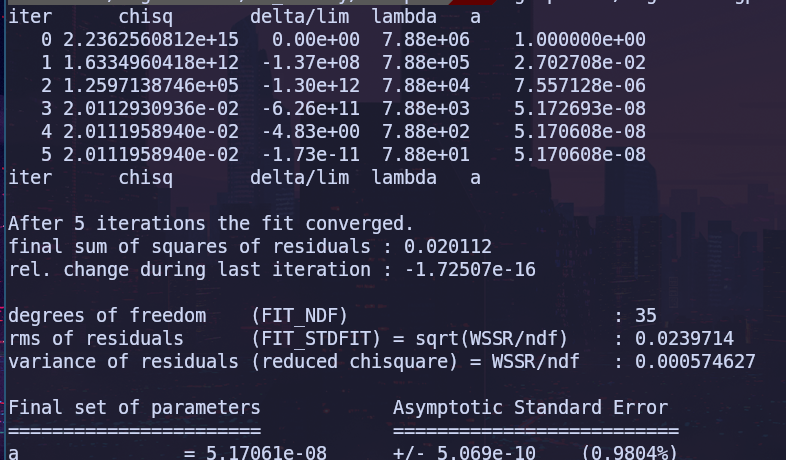
\includegraphics[scale = 0.40]{Problema1/Imagenes/FitLog.png}
    \end{subfigure} \hfill
    \begin{subfigure}{0.4\textwidth}
        \centering
        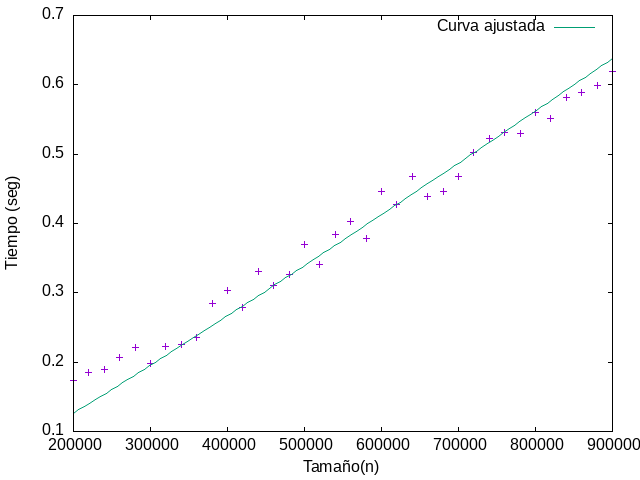
\includegraphics[scale = 0.40]{Problema1/Imagenes/regresion.png}
    \end{subfigure}
    \end{figure}

    Como podemos ver con este ajuste la varianza residual es prácticamente nulo y concuerda con los resultados teóricos, pudiendo así concluir que efectivamente nuestro algoritmo es del orden $O(n\log(n))$.



\newpage

\section{P2 Problema de asignación de aulas}

\subsection{Diseño del algoritmo}

\subsubsection{Descripción del problema}

     En una escuela se tiene que programar n exámenes en un día determinado, y para cada examen, disponemos de su tiempo de inicio y su duración. El centro cuenta con m aulas disponibles, donde m es mayor que N, asegurando así la posibilidad de realizar todos los exámenes incluso en el peor caso.
     Pero para cada aula reservada se necesita contratar a un vigilante 
     para supervisar dicha aula. Por tanto, se nos pide diseñar un algoritmo que permita garantizar que los exámenes se realicen con el menor costo posible para la escuela, es decir, reservando el
     menor número de aulas posibles.

\subsubsection{Algoritmo greedy}

    Proponemos una solución al problema que consiste en, una vez ordenados los exámenes según orden de inicio, ir reservando primero aulas para los exámenes que más pronto empiecen. Teniendo en cuenta de que si para el inicio de un examen existe una aula de las ya reservadas que esté libre, entonces se usa dicha aula, en caso contrario, se reserva otra nueva.
    Notemos que al ir reservando aulas primero para los exámenes que más pronto empiecen, a la hora de reservar aulas para un determinado examen, no va a haber exámenes para los cuales ya se ha reservado aula que empiece después del dicho examen.

    Este algoritmo es claramente greedy por el hecho de que toma decisiones locales para solucionar el problema completo y además en cada desión procura reservar el menor número de aulas posible. \\

    
\subsubsection{Componentes y demostración de validez}

    Veamos a ver los aspectos que hay que tener en cuenta en el diseño del algoritmo voráz:

    \begin{itemize}
        \item \textbf{Conjunto candidato: } Todas las aulas disponibles. Dentro de todas las aulas, seleccionaremos un número determinado de aulas.
        \item  \textbf{Conjunto seleccionado: } Las aulas seleccionadas que van ser usadas para realizar los exámenes, que también conforman la solución al problema a resolver.
        \item \textbf{Función solución: } Para que el conjunto seleccionado sea una solución al problema, este debe poder garantizar que se pueda realizar todos los exámenes en su tiempo 
        establecido, así, la función solución debe comprobar que si con las aulas seleccionadas se han podido programar todos los exámenes, independientemente de que sea el óptimo o no.
        \item \textbf{Función selector: } La función selector seleccionará una aula para un examen según el criterio de nuestro algoritmo. 
        \item \textbf{Función de factibilidad: } La función de factibilidad comprobará si la aula seleccionada para el examen
        es compatible con el resto de exámenes ya seleccionadas, es decir, que no haya dos exámenes que se vayan a realizarse en una misma aula en un mismo tiempo, independientemente de que sea el óptimo o no.
        \item \textbf{Función objetivo: } La función objetivo debe indicar el número de aulas seleccionadas, así como la programación de los exámenes.
        
    \end{itemize}

    Ahora vamos a demostrar por inducción que nuestro algoritmo encuentra el número mínimo de aulas necesarias (m aulas) para realizar todos los exámenes (n examenes), con $ m \leq n $. Veamos:

    \begin{itemize}
        \item \textbf{CASO BASE: (n = 1): } Nuestro algoritmo seleccionaría el primer examen que empieza y es claro que como tenemos uno solo, y este se tiene que realizar, necesitamos reservar un aula. Por tanto, es obvio que este es el óptimo y coincide con la elección de nuestro algoritmo.

        \item \textbf{PASO DE INDUCCIÓN: } Supongamos que nuestro algoritmo para los n exámenes que empiezan primero ha reservado m aulas, y este es el óptimo por hipótesis de inducción. Supongamos ahora que se necesita hacer un examen más (el n+1-ésimo), que es el siguiente según el tiempo de comienzo, entonces según nuestro algoritmo: \\
        \begin{itemize}
            \item Si alguna de las aulas reservadas está ya libre para la hora de comienzo del examen n+1-ésimo, entonces realizaremos en esta aula el dicho examen. Por tanto, habremos reservado hasta el momento m aulas que era el óptimo para n éxamenes, luego al no aumentar el número de aulas, es claro que este es óptimo también.
            \item Si todas las aulas reservadas hasta el momento del comienzo del examen n+1-ésimo están ocupadas, entonces nuestro algoritmo reservará otra aula. Por tanto, tendremos m+1 aulas reservadas. Por reducción al absurdo probemos que este es el número óptimo. \\
            Si existiese otra solución que reserve menos aulas para n+1 exámenes siendo $\bar{m}$ el número de aulas que se reserva, entonces tenemos que $\bar{m} < m+1$. Pero como para el comienzo del examen n+1-ésimo todas las m aulas estaban ocupadas, deducimos que había m exámenes realizándose, por tanto, para el inicio del n+1-ésimo habrá m+1 exámenes en proceso. Entonces, como la solución óptima debe permitir que se realicen todos los exámenes, en particular al comienzo del examen n+1-ésimo, entonces $ m + 1 \leq \bar{m}$. Juntando las desigualdades tenemos $ m + 1 \leq \bar{m} < m + 1$, contradicción. Luego m + 1 aulas era el óptimo para este caso.
        \end{itemize}
        
    \end{itemize}

    Y así, concluimos con que nuestro algoritmo nos da el mínimo número de aulas a reservar para realizar n exámenes, siendo n un número natural arbitrario, es decir, para cualquier número número de exámenes nuestro algoritmo nos da el óptimo número de aulas.

\subsection{Implementación y estudio de eficiencias: }

\subsubsection{Datos de entrada y evaluación de validez: }

\myparagraph{Formato datos entrada: }
    Como entrada necesitaremos el número de exámenes a planificar así como 
    la información relativa a cada examen, es decir, la hora de inicio y 
    la duración de cada uno. Para esto último hemos decidido que el formato de la hora de inicio será de la forma horas:minutos (ej. 15:30) y la duración será expresado en minutos. A continuación 
    mostraremos un ejemplo: 

    \begin{verbatim}
    4
    6:00 30
    6:10 30
    6:30 20
    6:40 20
    \end{verbatim}
    
\subsubsection{Implementación: }
    A continuación mostramos la implementación del algoritmo descrito anteriormente: 

    En primer lugar tenemos una estructura $info\_exam$ para gestionar la información relativa a un examen así como conversión entre formatos de tiempo y E/S. Es fácil ver que todos los métodos implementados son de orden constante, es decir, O(1).
    
    \lstinputlisting[language=C++, firstline=10,lastline=155]{Problema2/codigos/greedy.cpp}

    A continuación mostramos el algoritmo en sí:
    
    \lstinputlisting[language=C++, firstline=160,lastline=215]{Problema2/codigos/greedy.cpp}
    
    Como dijimos, el algoritmo en primer lugar ordena el vector y seguido
    selecciona para cada examen un aula según el criterio establecido.
    Para ello, mantiene un priority\_queue o heap donde guarda récord del último examen que se va a realizar en cada aula en el momento, y en el 
    tope está el examen que acaba más proto, facilitando así la elección
    de aulas.Si el del tope no ha acabado, el resto tampoco habrán 
    acabado, por tanto hay que reservar nuevas aulas. Sin embargo, si el 
    del tope ha acabado entonces ya disponemos de un aula y no hay que reservar más aulas.
    
    En el main podemos ver la función objetivo que imprime la programción
    de los exámenes por completo si está definida la macro PROGRAMACION
    e imprime solo el número de aulas necesarias si está definida la macro 
    NUM\_AULAS:

    \lstinputlisting[language=C++, firstline=252,lastline=293]{Problema2/codigos/greedy.cpp}

    Un ejemplo de la ejecución con opción PROGRAMACIÓN sería: 

    \begin{verbatim}
    Entrada:      
    4
    6:00 30
    6:10 30
    6:30 20
    6:40 20
    
    Salida:  
    Classroom 0 : 
    [6:00,30 min] [6:30,20 min] 
    Classroom 1 : 
    [6:10,30 min] [6:40,20 min] 
    
    \end{verbatim}

    \subsubsection{Estudio de eficiencia: }

    \myparagraph{Eficiencia teórica: }

    Estudiemos la eficiencia teórica. En primer lugar, la ordenación es del orden $O(n \log (n))$. Seguido, en el bucle se realizan n iteraciones, siendo n el número de exámenes. Ahora, cuando se busca una potencial aula vacía de las ya reservadas solo tenemos que consultar el tope del heap, puesto que ese será el primer examen que acabe dentro de los que se están realizándose. Teniendo en cuenta que en el peor de los casos el heap puede tener i exámenes en cada iteración y la inserción en un heap es del orden logarítmico, concluimos que el orden del bucle for es $O(n \log (n))$, ya que el resto de sentencias en ambos condicionales son operaciones simples de orden $O(1)$. Por tanto, aplicando la regla de la suma y del máximo la eficiencia teórica del algoritmo es $O(n \log (n))$. 
    
    Notemos que este algoritmo obtiene la programación completa de los exámenes, pero eso es equivalente a obtener el número de aulas mínimo, 
    puesto que basta obtener el tamaño del vector solución. Propondremos otra alternativa más eficiente teóricamente pero que no nos ofrece 
    una información tan completa como el estudiado en esta sección.

    \myparagraph{Eficiencia empírica e híbida: }
    
    En cuanto a la eficiencia empírica, ejecutando casos de 37000-2600000 exámenes con el formato descrito anteriormente, obtenemos las siguientes gráficas:

    \begin{figure}[H]
    \begin{subfigure}{0.4\textwidth}
        \centering
        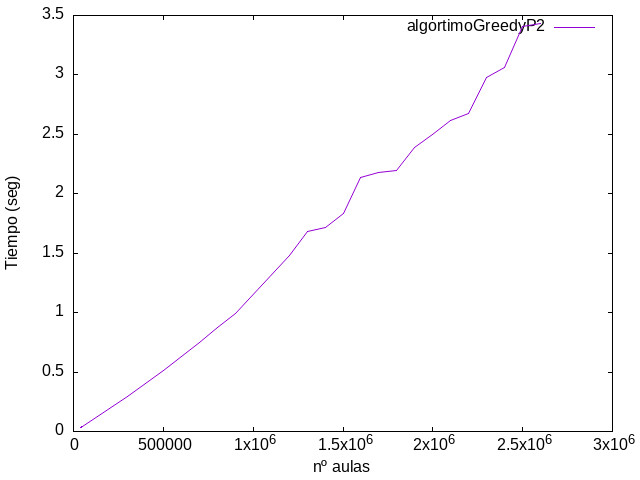
\includegraphics[scale = 0.40]{Problema2/imagenes/GraficaLineas.jpeg}
    \end{subfigure} \hfill
    \begin{subfigure}{0.4\textwidth}
        \centering
        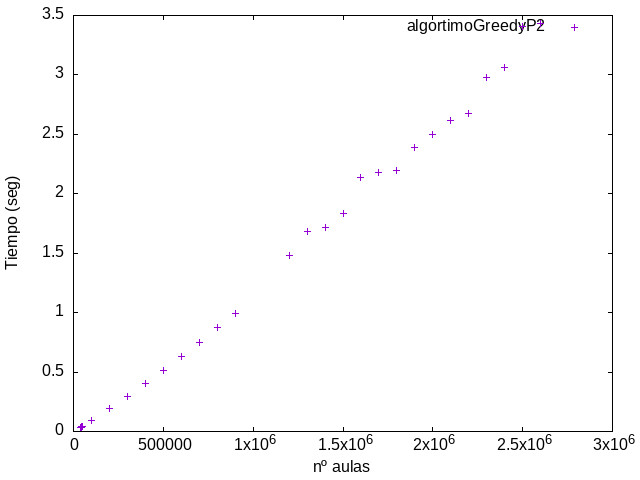
\includegraphics[scale = 0.40]{Problema2/imagenes/GraficaPuntos.jpeg}
    \end{subfigure}
    \end{figure}

    Como podemos ver, aunque haya leves fluctuaciones podemos ver que tiene un crecimiento casi lineal, y si lo ajustamos con una curva de 
    regresión del tipo $a_0 n \log (n)$ obtemos los siguientes resultados: 

    \begin{figure}[H]
    \begin{subfigure}{0.4\textwidth}
        \centering
        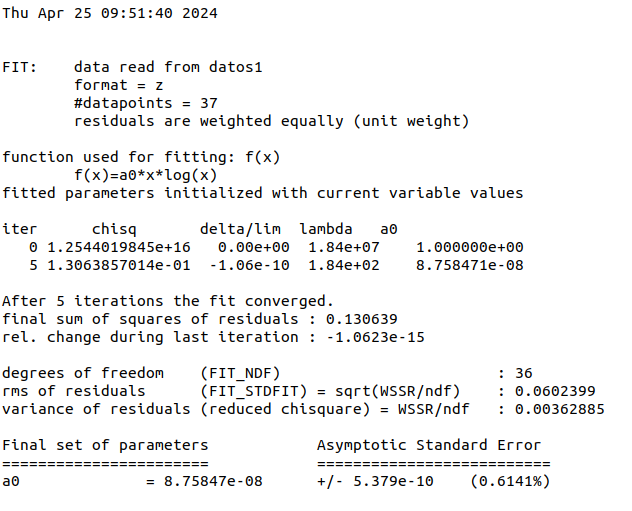
\includegraphics[scale = 0.40]{Problema2/imagenes/fitLog.png}
    \end{subfigure} \hfill
    \begin{subfigure}{0.4\textwidth}
        \centering
        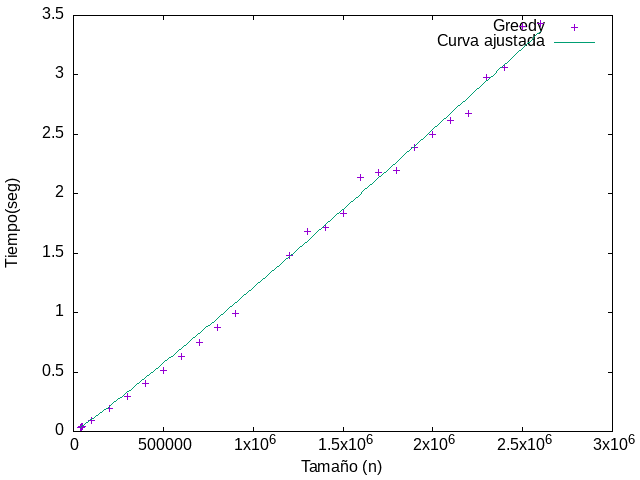
\includegraphics[scale = 0.40]{Problema2/imagenes/Salida_ajustada1.jpeg}
    \end{subfigure}
    \end{figure}

    Como podemos ver con este ajuste la varianza residual es practicamente nulo y concuerda con los resultados teóricos, pudiendo así concluir que efectivamente nuestro algoritmo es del orden $O(n\log(n))$.

    \subsubsection{Alternativas: }
    Aquí presentamos una solución alternativa que obtiene solo el número de aulas a reservar con eficiencia $O(n \log (n))$ también, con n el número de examenes a realizar: 
    
    \lstinputlisting[language=C++, firstline=153,lastline=186]{Problema2/codigos/checker.cpp}

    Notemos que también es una solución greedy, puesto que max\_count, que es el número de aulas a reservar, no reserva más aulas hasta que se necesite más aulas de las que se han reservado hasta el momento. 
    La idea de este algoritmo es saber que el mínimo número de aulas a reservar coincide con el máximo de examenes que se solapan en el tiempo. 
    
\newpage
\section{struct City}

Para resolver los problemas 3 y 4 con mayor comodidad y facilitar la modularización y legibilidad del código, se ha hecho uso de una  $struct$ $City$ para representar las ciudades del problema.
\lstinputlisting[language=C++, firstline=7,lastline=9]{Problema4/codigos/City.h}
Se ha definido también una constante $INF$ para representar un valor de distancia imposible mayor que cualquier otro de los que pueda haber dentro del problema.
\lstinputlisting[language=C++, firstline=9,lastline=11]{Problema4/codigos/City.h}
%\lstinputlisting[language=C++, firstline=14,lastline=62]{Codigos/P3/City.h}

La $struct$ $City$ representa las ciudades del problema mediante sus coordenadas $(x,y)$.\\
\lstinputlisting[language=C++, firstline=16,lastline=18]{Problema4/codigos/City.h}
Además implementa la función $dist$ que calcula la distancia euclídea de una ciudad a otra y tiene sobrecargado el operador $-$ para este mismo propósito.
\lstinputlisting[language=C++, firstline=23,lastline=32]{Problema4/codigos/City.h}

El operador $<$ también ha sido sobrecargado puesto que en nuestros algoritmos nos valimos de ordenar las ciudades respectod el eje $x$ para dar con soluciones más óptimas y eficientes.

\lstinputlisting[language=C++, firstline=34,lastline=43]{Problema4/codigos/City.h}

Por último se han sobrecargado los operadores distinto ($!=$) y igual ($==$) por comodidad a la hora de trabajar con $City$ y los operadores de entrada ($>>$) y salida ($<<$) para facilitar la lectura y escrituda de datos.

\lstinputlisting[language=C++, firstline=45,lastline=62]{Problema4/codigos/City.h}

Para finalizar, se ha implementado la función $printCycle()$ la cual recibe como parámetros el orden de los índices de las ciudades, la ciudad de origin y un array con las ciudades e imprime las ciudades empezando y acabando en la ciudad de origen en el orden indicado. Esto se ha hecho para facilitar la impresión de ciudades en el orden correcto teniendo en cuenta que el array de ciudades original ha sido ordenado.

\lstinputlisting[language=C++, firstline=103,lastline=113]{Problema4/codigos/City.h}
\newpage
\section{P3: Problema del camino mínimo}
\subsection{Definición del problema}
Tenemos un conjunto de n ciudades (puntos en un plano), cada una definida por las coordenadas en el mapa $(x_i, y_i)$, con $i = 1, . . . , n$. Cada ciudad se puede conectar por carretera con
un subconjunto de ciudades, asegurando que la red de vías que se genere crea un grafo conexo.

La distancia entre dos ciudades viene dada por la distancia euclídea entre sus coordenadas.

\[
    dist((x_1,y_1),(x_2,y_2)) = \sqrt{(x_1-y_1)^2+(x_2-y_2)^2}
\]

Dada una ciudad de origen, $x$, y una ciudad de destino, $y$, se pide encontrar el camino de
costo mínimo que permita viajar de $x$ a $y$.
\subsection{Diseño del algoritmo}
\subsubsection{Algoritmo Greedy}
La solución que se describe a este problema se le conoce como algoritmo de Dijkstra, el cual es muy útil para calcular la distancia mínima en un grafo de un nodo a cualquier otro. En este caso concreto se ha modificado ligeramente para también guardar el camino mínimo. El algoritmo consiste en, partiendo de la ciudad origen $x$, y de que su distancia mínima a cualquier ciudad por el momento es $+\infty$, comprobar su distancia a las ciudades adyacentes (las que estén conectadas por carretera directa) y actualizarla. Luego para cada una de esas ciudades (llamémoslas ciudades intermedias), y para cada una de sus ciudades adyacentes, se comprueba si el camino hacia ellas pasando por la ciudad intermedia es menor que el original que teníamos, actualizando el camino mínimo. Este proceso se repite hasta que ya no queden más ciudades que explorar (habremos explorado todas las ciudades pues se parte de que el grafo es conexo). Para guardar además el camino hacia cada ciudad cada ciudad tendrá asociada en todo momento su ciudad previa en el camino mínimo, y se irá actualizando conforme sea necesario.

\subsubsection{Componentes y demostración de validez}

Las componentes del algoritmo greedy son:

\begin{itemize}
    \item \textbf{Conjunto candidatos V:} Todos las ciudades de la instancia del problema
    \item \textbf{Conjunto seleccionados S:} Todas las ciudades para las cuales ya se conoce el camino mínimo.
     \item \textbf{Función selección:} En cada paso se añade el nodo con menor coste de entre los no seleccionados \verb|V\S| al conjunto de seleccionados.
\end{itemize}
A continuación demostraremos por inducción la validez del algoritmo de Dijkstra para el cálculo de caminos mínimos. 

La demostración es por inducción.

\begin{itemize}
    \item \textbf{Caso base} ($|S|=0$): trivial
    \item \textbf{Paso de inducción:} Supongamos que para todo nodo del conjunto \verb|S| se conoce su distancia mínima al nodo origen $s$ que es la calculada por el algoritmo de Dijkstra $d(u)\ \forall u \in S$. Ahora supongamos que el algoritmo de Dijkstra añade un nodo $v$ al conjunto $S$. Demostremos por reducción al absurdo. Supongamos que la distancia a $v$ calculada por el algoritmo de Dijkstra $d(v)$ no es la mínima. Entonces sea $P$ el camino mínimo desde $s$ hasta $v$, y su peso notado como $M(s,v)$. Ahora sea $x$ el último nodo del camino $P$ antes de salirse de $S$ (todos los anteriores son de $S$ y el siguiente no). Sea $y$ el nodo inmediatamente posterior a $x$ en $P$. Sea entonces $c(x,y)$ el peso del arco $(x,y)$. Se tiene que:
\[
    d(v) > M(s,v) = M(s,x) + c(x,y) + M(y,v) \geq M(s,x) + c(x,y) = d(x) + c(x,y) \geq d(y)    
\]
    Donde en la primera desigualdad hemos usado la suposición de la reducción al absurdo, en la primera igualdad hemos usado que el problema tiene subestructuras optimales, en la segunda igualdad hemos usado la hipótesis de inducción y la última desigualdad se debe a que no hay pesos negativos.

    En definitiva, se ha llegado a que $d(v) > d(y)$, lo cual es una contradicción pues en cada paso el algoritmo de Dijkstra escoge al nodo con menor distancia al conjunto, por lo que el algoritmo de Dijkstra hubiera seleccionado al nodo $y$ en lugar del nodo $v$. Ello viene de suponer que $d(v) > M(s,v)$, por lo que queda demostrado que $d(v) = M(s,v)$.

\end{itemize}

\subsection{Implementación y estudio de eficiencia}
\subsubsection{Datos de entrada}
El formato de entrada de datos que hemos seguido es el que se muestra en la siguiente función main: 
\lstinputlisting[language=C++, firstline=80,lastline=147]{Problema3/codigos/greedy.cpp}

Los datos de entrada se leen desde un fichero (instancias) que se pasa como parámetro al programa y que contiene los datos en el formato que se muestra comentado en el código:
Primero lee un entero $N$ que será el número de ciudades del problema. Luego lee dos enteros entre $0$ y $N-1$ que representarán el número de ciudad de origen y destino, respectivamente, de entre las $N$ ciudades que se pasan a continuación, en el formato que indica el operador de entrada del \texttt{struct City.h}. Con esto ya se leen las ciudades, a continuación se pasan a leer las aristas del grafo (carreteras). Primero se lee el número de aristas que tiene el grafo $M$ y a continuación se leen $M$ pares de enteros que representan los números asociados a cada ciudad (según el orden en el que se habían introducido, empezando por 0) que indican que en el grafo hay una arista que contiene a esos dos nodos (una carretera que une esas dos ciudades). 

El grafo se representa mediante un vector de vectores, en el que el vector \texttt{roads[i]} contiene todas las ciudades con conexión directa con la ciudad \texttt{cities[i]} así como sus respectivas distancias. 

\subsubsection{Implementación}
A continuación se explica la implementación del algorimo de Dijkstra en detalle el cuál es llamado en la línea 57 de la función main:

\lstinputlisting[language=C++, firstline=37,lastline=78]{Problema3/codigos/greedy.cpp}

Los parámetros de la función son, el grafo de ciudades y carreteras, que ahora serán referidos como nodos y aristas, como parámetro de entrada; un vector \verb|dist| de manera que al final de la función \verb|dist[i]| guardará la distancia mínima desde el nodo \verb|origin| hasta el nodo \verb|i|; un vector \verb|prev| de manera que en el camino mínimo desde \verb|origin| hasta \verb|i|, antes de llegar a \verb|i|, se pasa por \verb|prev[i]|; y por último el parámetro de entrada \verb|origin| como el nodo origen a partir del cual se calculará el camino mínimo a cada nodo.

Comenzamos por declarar una cola con prioridad \verb|q| que tendrá siempre al frente el siguiente nodo a seleccionar:

\lstinputlisting[language=C++, firstline=11,lastline=12]{Problema3/codigos/greedy.cpp}

Después, se guarda en la cola el primer nodo \verb|origin| con distancia 0, que también se guarda en \verb|dist|.

A continuación, se entra en un bucle en el cual se procesa siempre el elemento \verb|p| con menor distancia a \verb|origin| (el primero de la cola \verb|q|), empezando claro está por el mismo \verb|origin|, tomando solo su índice \verb|node| (la distancia no hace falta pues ya la tendremos en \verb|dist[node]|). Y ahora para cada nodo \verb|u| adyacente a \verb|node| tomamos su índice \verb|v| y su distancia actual \verb|d| a \verb|origin| (si no se ha procesado, será $+\infty$), y comparamos el peso del camino pasando por \verb|node| y de \verb|node| a \verb|v| con el peso del camino actual a \verb|v| (línea 31) y en caso de que sea menor (la primera vez que se procese siempre lo será) se actualiza el peso del camino a \verb|v|, \verb|dist[v]| y por tanto el previo a \verb|v| en su camino mínimo \verb|prev[v]|. Por último, se añade el nodo de índice \verb|v| con su distancia actualizada \verb|dist[v]| a la cola \verb|q| para procesarlo en futuras iteraciones del bucle. Se añadirán a la cola aquellos nodos para los que se haya encontrado un camino más corto pasando por el nodo intermedio (\verb|node|) por lo que no hay que preocuparse de casos como que se añadan dos nodos en bucle infinito a la cola al ser la distancia una función positiva. Si hubiese pesos negativos se podría dar una situación como la anterior.

\subsubsection{Estudio de eficiencia}

\myparagraph{Eficiencia teórica:}

Analizamos el algoritmo para la eficiencia teórica. En el bucle externo, primero eliminamos el nodo al frente del heap, lo cual tiene una eficiencia de $O(log\ n)$ siendo $n$ el número de nodos. El bucle for interno se ejecuta un máximo de $n$ veces y dentro de él se elimina el nodo $v$ del heap en caso de que sea mejor el camino por $node$. Esto no ocurre más de una vez por arista. Por tanto el algoritmo de Dijkstra tiene una eficiencia del orden de $O((a+n)log\ n)$ siendo $a$ el número de arcos y $n$ el número de nodos. Si nos reducimos al caso de un grafo conexo, que es el nuestro, tenemos que $a \geq n-1$ y por tanto la eficiencia pasa a ser $O(a\ log\ n)$. En el caso de grafos muy densos, la versión de cola con prioridad pierde eficiencia, pues en el caso de un grafo completo sería del orden de $O(n^2\ log\ n)$.

\myparagraph{Eficiencia empírica e híbrida:}

Al ejecutar para diferentes números de ciudades el programa (desde 5000 hasta 125000) obtenemos los siguientes tiempos de ejecución:

\begin{center}
    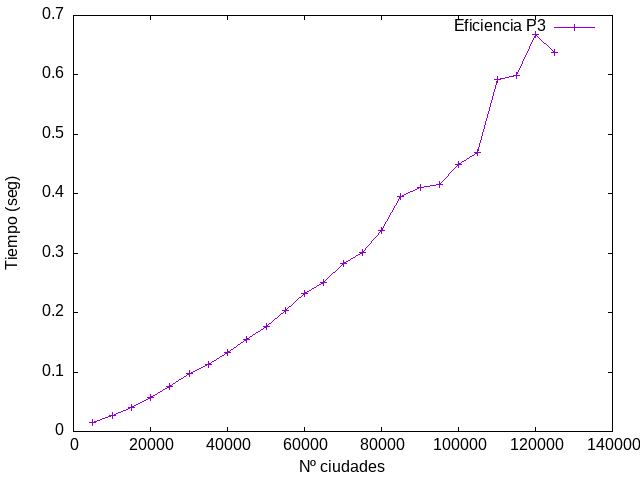
\includegraphics[width=0.7\textwidth]{Problema3/imagenes/timesP3.png}   
\end{center}

Se puede observar que no sigue una curva uniforma (una cuadrática o una lineal-logarítmica) ya que la eficiencia depende también del número de arcos, que es generado aleatoriamente entre $n-1$ para que sea conexo y $n^2$.

Si tratamos de hacer una regresión cuadrática o lineal logarítmica obtenemos los siguientes resultados.

\begin{figure}[H]
    \begin{subfigure}{0.5\textwidth}
        \centering
        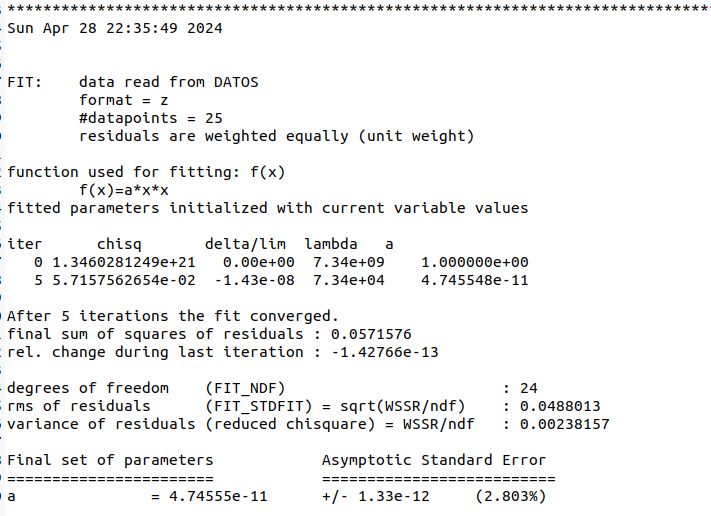
\includegraphics[width=\textwidth]{Problema3/imagenes/log-cuadratico.png}
    \end{subfigure} \hfill
    \begin{subfigure}{0.5\textwidth}
        \centering
        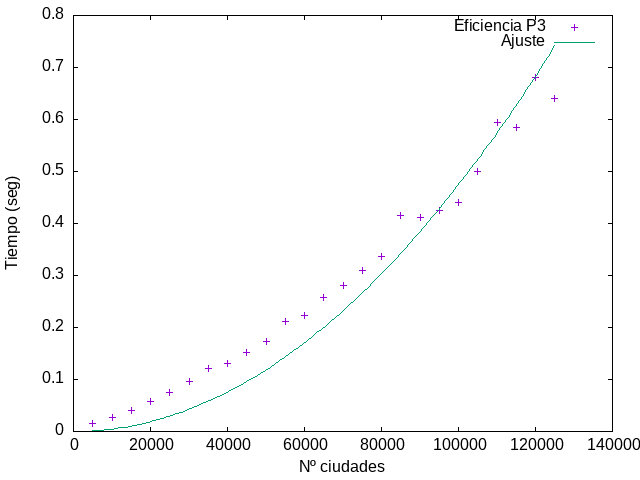
\includegraphics[width=\textwidth]{Problema3/imagenes/regresionP3.png}
    \end{subfigure}
\end{figure}

\begin{figure}[H]
    \begin{subfigure}{0.5\textwidth}
        \centering
        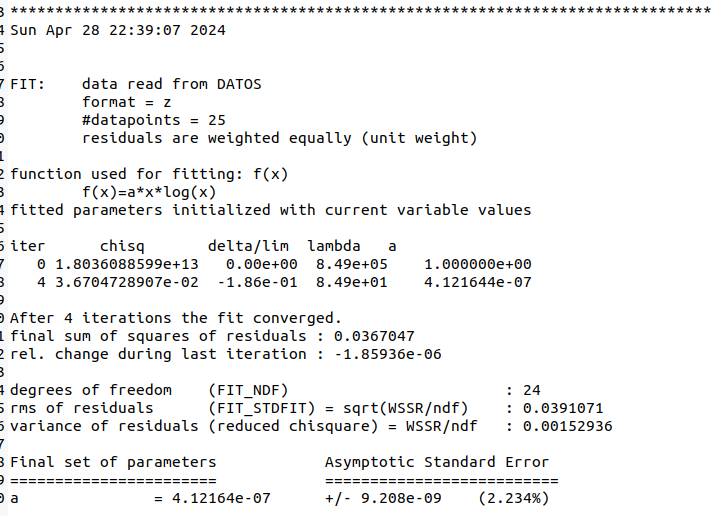
\includegraphics[width=\textwidth]{Problema3/imagenes/log-lin-log.png}
    \end{subfigure} \hfill
    \begin{subfigure}{0.5\textwidth}
        \centering
        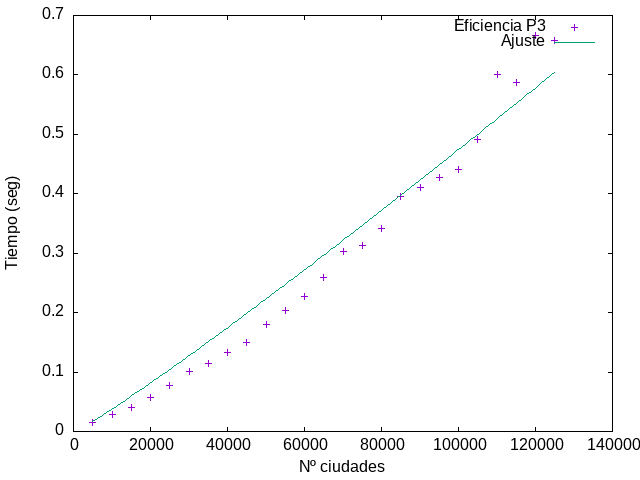
\includegraphics[width=\textwidth]{Problema3/imagenes/regresion-lin-logP3.png}
    \end{subfigure}
\end{figure}

Observamos que con ambos ajustes se obtiene un error no despreciable porque el número de aristas, que se está tomando de forma arbitraria, se tiene en cuenta también a la hora de calcular la eficiencia.

\newpage
\section{P4: Problema del Viajante de Comercio}
\subsection{Definición del problema}
Tenemos un conjunto de $n$ ciudades (puntos en un plano),
cada una definida por las coordenadas en el mapa $(x_i, y_i)$,
con $i = 1,\ ...\ , n$. La distancia entre dos ciudades viene
dada por la distancia euclídea entre sus coordenadas.
\[
dist((x_1, y_1),(x_2, y_2)) = \sqrt{(x_1 - x_2)^2 + (y_1 - y_2)^2}
\]

El problema de viajante de comercio consiste en encontrar el
orden en el que un viajante, partiendo de la ciudad de origen
(por ejemplo $(x_1, y_1)$) pase por todas y cada una de las ciudades
una única vez, para volver a la ciudad de partida, formando un ciclo.

El costo del ciclo será la suma de las distancias que hay entre todas las ciudades consecutivas.

El problema original del viajante de comercio consiste en encontrar el ciclo de costo mínimo entre todas las posibilidades existentes.

Aunque este problema es NP-Difícil y por tanto no podemos esperar
encontrar una solución óptima al mismo, lo que se pretende en esta
práctica es utilizar la estrategia del greedy
para encontrar una solución aproximada que puede ser de utilidad en
situaciones como las que se plantea en este problema.

\myparagraph{Input/Output}

Se ha tomado como datos de entrada un entero $n$ indicando el número de ciudades a visitar, seguido de $n$ líneas, cada
una representando las coordenadas de la ciudad en cuestión
siguiendo el siguiente formato: $(x,y)$ donde $x$ es un 
número en coma flotante que representa la posición de la ciudad
en el eje X e $y$ es lo mismo para el eje Y.

La salida del programa consiste en $n+1$ líneas cada una 
representando las coordenadas de la ciudad en cuestión según el
formato previamente especificado. La primera y última
siempre contienen las coordenadas de la ciudad de origen.
En general, representan un camino donde si se está en la 
ciudad de la línea i-ésima después se va a la ciudad de 
la línea (i+1)-ésima.

\begin{ejemplo}
    
\end{ejemplo}

\subsection{Versión 1}
\subsubsection{Diseño e implementación del algoritmo voraz}
\myparagraph{Diseño}

La primera versión de algoritmo greedy para resolver este problema es la más sencilla de todas, y es la que se le puede ocurrir a uno de forma más directa, aplicando la heurística ($greedy$) a los nodos del grafo. Se trata de en cada paso ir a la ciudad más cercana (closest neighbour) hasta que hayamos visitado todas las ciudades.

Dado que el problema es NP-Difícil, esta estrategia no da con la solución óptima, pero sí es cierto que consigue un resultado aproximado de manera fácil y rápida.

\myparagraph{Implementación}
\lstinputlisting[language=C++, firstline=38,lastline=72]{Problema4/codigos/greedy_v1.cpp}

En la función, \verb|n| es un entero que indica el número de ciudades y \verb|home_ind| indica el índice la ciudad desde la que se parte en el vector \verb|v|, que almacena todas las ciudades haciendo uso de la \verb|struct City|. Finalmente, la solución se va guardando en forma de secuencia de índices en el vector \verb|path|, que tendrá como primer y último elemento a \verb|home_ind|.

\vspace{0.5cm}

Se comienza inicializando un vector que guardará los índices de las ciudades que no se hayan visitado. Este vector irá decreciendo en tamaño durante la ejecución de la función. A continuación se inicializa dicho vector con las ciudades en orden y se declara \verb|current| a \verb|home_ind|, donde \verb|current| indicará en todo momento la ciudad que se está visitando. Después en cada iteración del bucle se añade la ciudad actual a \verb|path| y se elimina de \verb|not_visited|. Luego, para cada ciudad de entre todas las ciudades no visitadas se calcula aquella con menor distancia a la actual, y se selecciona para la siguiente iteración.

\vspace{0.5cm}

La función \verb|remove| es la que se muestra a continuación:

\lstinputlisting[language=C++, firstline=22,lastline=28]{Problema4/codigos/greedy_v1.cpp}

Eficiencia de remove: lineal.

\subsubsection{Análisis de eficiencia}
\myparagraph{Eficiencia teórica}

La eficiencia teórica es sencilla en este caso. Para cada ciudad, se elimina la ciudad del vector de no visitados en orden lineal, y se calcula la distancia mínima en el orden del número de ciudades que queden por visitar. Aplicando la regla del máximo, visitar cada ciudad supone un costo lineal, y como se visitan todas las ciudades el orden de eficiencia es $O(n^2)$.

\myparagraph{Eficiencia empírica}

Al ejecutar el programa para números de ciudades desde 500 hasta 12500 con saltos de 500 se obtienen los siguientes resultados:

\begin{center}
    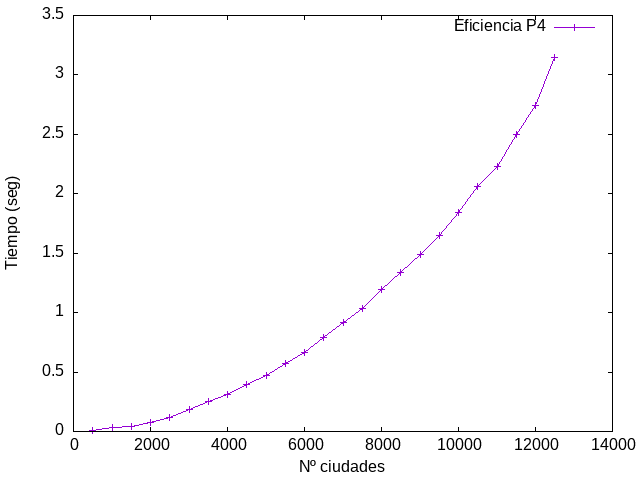
\includegraphics[width=0.7\textwidth]{Problema4/imagenes/timesP4.png}   
\end{center}

\myparagraph{Eficiencia híbrida}

A la hora de hacer un ajuste cuadrático se obtiene el siguiente resultado.

\begin{figure}[H]
    \begin{subfigure}{0.5\textwidth}
        \centering
        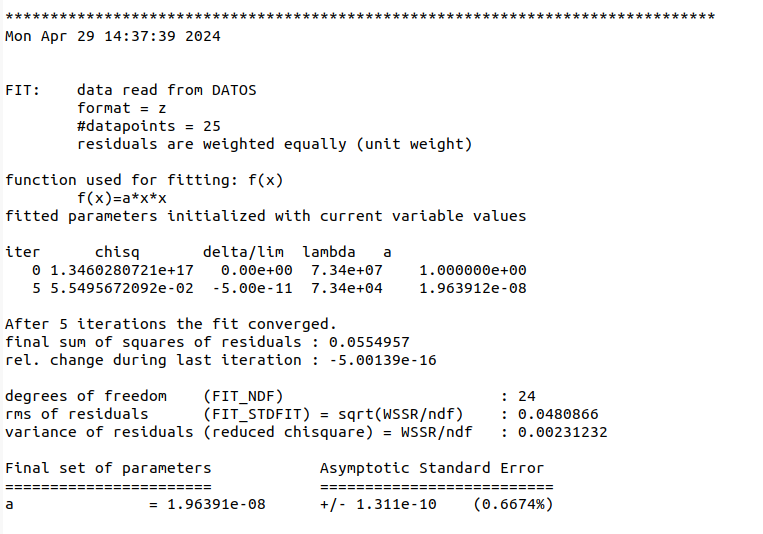
\includegraphics[width=\textwidth]{Problema4/imagenes/logP4.png}
    \end{subfigure} \hfill
    \begin{subfigure}{0.5\textwidth}
        \centering
        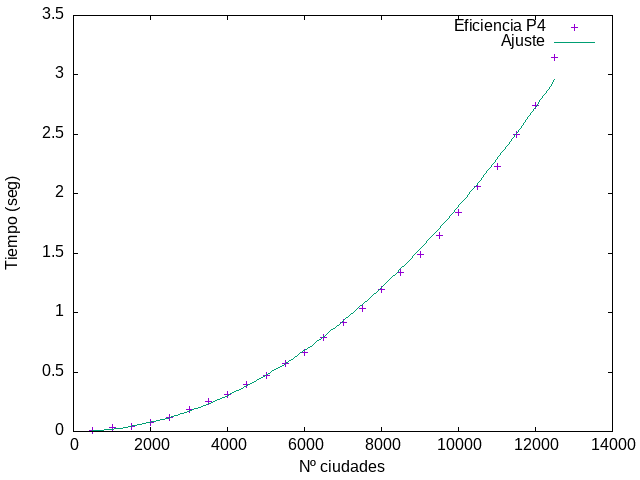
\includegraphics[width=\textwidth]{Problema4/imagenes/regresion_cuadraticaP4.png}
    \end{subfigure}
\end{figure}

La función obtenida es:

\[
    f(x) = 1.96391 \cdot 10^{-8} \cdot x
\]

La cual como vemos, se ajusta prácticamente a la perfección a la gráfica obtenida, reafirmando nuestra conclusión en el análisis teórico de que la eficiencia de la función es $O(n^2)$.

\subsection{Versión 2}
\subsubsection{Diseño e implementación del algoritmo voraz}
\myparagraph{Diseño}
En esta versión de la solución, hemos optado por aplicar la heurística voraz ($greedy$) a los arcos del grafo en vez de a los nodos, al contrario de la versión anterior. La solución se resume en dos sencillos sencillos pasos:
\begin{enumerate}
    \item Construir el árbol recubridor mínimo (\textit{Minimum Spanning Tree o \textbf{MST}}).
    \item Listar el árbol construido en preorden, transformándolo así en un ciclo que recorre todas las ciudades una única vez.
\end{enumerate}
\begin{ejemplo}
Dadas las siguientes ciudades y sus coordenadas:
\begin{figure}[H]
    \centering
    \begin{subfigure}{0.3\textwidth}
    \begin{verbatim}
        10
        (0.61093,0.565811)
        (0.179647,0.505768)
        (0.183472,0.816686)
        (0.422156,0.584653)
        (0.31626,0.0253342)
        (0.083659,0.0612762)
        (0.978058,0.976791)
        (0.0530768,0.873889)
        (0.0923382,0.268988)
        (0.562573,0.880963)
    \end{verbatim}
    \caption{Input data}
    \end{subfigure}
    \hfill
    \begin{subfigure}{0.45\textwidth}
        \centering
        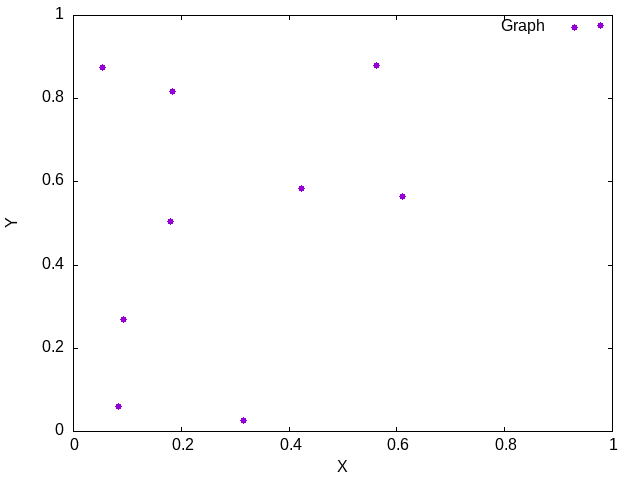
\includegraphics[width=\textwidth]{Problema4/imagenes/example_graph.png}
        \caption{Representación gráfica}
        \label{fig:example_graph}
    \end{subfigure}
\end{figure}
\end{ejemplo}
Obtenga el ciclo de coste mínimo que recorra todas las ciudades una única vez (partiendo y acabando en la primera ciudad).
\myparagraph{Solución}
\begin{figure}[!hbt]
    \centering
    \begin{subfigure}{0.45\textwidth}
        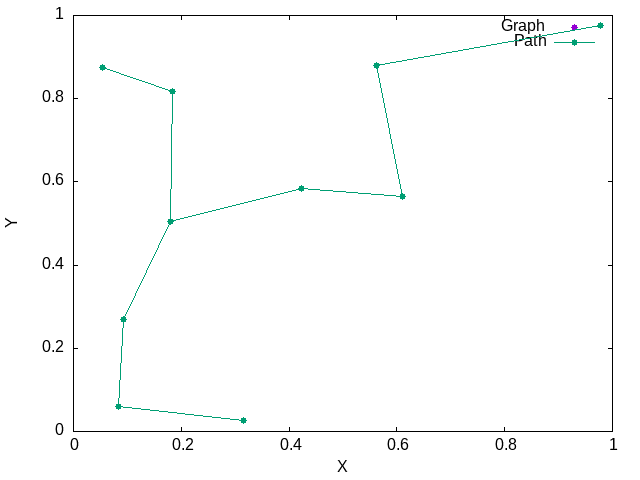
\includegraphics[width=\textwidth]{Problema4/imagenes/example_graph_mst.png}
        \subcaption{Árbol recubridor mínimo (MST)}
    \end{subfigure}
    \begin{subfigure}{0.45\textwidth}
        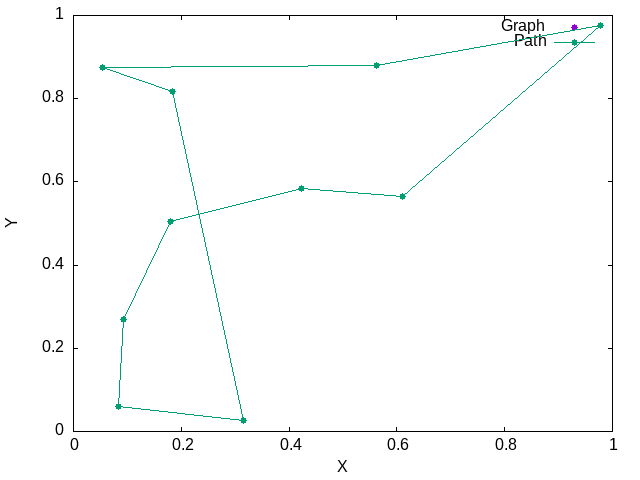
\includegraphics[width=\textwidth]{Problema4/imagenes/example_graph_sol_v2.png}
        \subcaption{Recorrido en preorden (solución)}
    \end{subfigure}
\end{figure}
\myparagraph{Calidad de la solución}

Si eliminamos un arco a la solución óptima del problema del viajante de comercio (llamémosla $TSP$), obtenemos un árbol.
Por definición de árbol recubridor mínimo (llamémosle $TSP$), sabemos que es el árbol cuya suma del peso sus arcos es mínima. Por tanto, dicha suma es menor que la suma del peso todos los arcos de $TSP$ menos uno, (y por tanto menor que la de todos).

Si quisiéramos recorrer todos los nodos del grafo con tan solo los arcos del $MST$, en el peor de los casos deberíamos recorrer cada arco dos veces. Este caso se daría si todos los nodos estuvieran conectados al mismo y partiéramos del nodo raíz como se puede observar en la figura (\ref{fig:grafo}).

\begin{figure}[hbt!]
    \centering
    \begin{tikzpicture}
        \node[draw, circle] (A) at (0,0) {};
        \node[draw, circle] (B) at (1,-1) {};
        \node[draw, circle] (C) at (-1,-1) {};
        \node[draw, circle] (D) at (0,-1) {};

        \draw (A) -- (B);
        \draw (A) -- (C);
        \draw (A) -- (D);
        \path (D) -- node[auto=false]{\ldots} (B);
    \end{tikzpicture}
    \caption{MST en el que hay que recorrer todos los arcos para recorrer todos los nodos}
    \label{fig:grafo}
\end{figure}

Como nuestra solución lo que hace es listar el $MST$ en preorden, tenemos pues que si un nodo tiene más de un hijo, a la hora de visitar el siguiente hijo, en vez de volver a recorrer el arco que une al hijo anterior con el padre para después recorrer el arco que une al padre con el siguiente hijo, nuestro algoritmo se limita a ir directamente de un hijo al otro.

Dado que nuestro problema en particular trabaja con la distancia euclídea, la cual cumple la \textbf{desigualdad triangular}, es decir, la distancia de ir de un nodo a otro es menor o igual que la de ir primero a un nodo intermedio para después ir al nodo destino. Formalmente sería
$$\forall u,v,w \in V \:\: dist(u,v) \leq dist(u,w) + dist(w,v) \:\: \text{  (Desigualdad Triangular)}$$ donde $V$ es el conjunto de los nodos del grafo.

Tenemos pues que haciendo uso de dicha desigualdad, el coste de la solución proporcionada por nuestro algoritmo es menor o igual que el coste de recorrer $MST$ dos veces. Y por definición de $MST$, esto es menor o igual que el coste recorrer la solución óptima dos veces, donde por coste entendemos la suma de las distancias. Matemáticamente, notando nuestra solución por $SOL$, tenemos
$$cost(SOL) \leq 2 \cdot cost(MST) \leq 2 \cdot cost(TSP)$$

En conclusión, tenemos que el coste de la solución dada por este algoritmo es, en el peor de los casos, \textbf{a lo sumo 2 veces el coste de la solución óptima}.
\begin{comment}
\begin{teo}
 Sea un grafo no dirigido ponderado completo G = (V,E,dist) donde V es un conjunto de nodos, E es un conjunto de arcos que relacionan estos nodos, el cual al ser G un grafo completo se tiene que $$E = \{e \in P(V) : |e| = 2\}$$ y dist es la función de asignación de pesos $dist: E \longrightarrow \mathbb{R}$ la cual le pedimos que verifique que $$\forall u,v,w \in V \:\: dist(u,v) \leq dist(u,w) + dist(w,v) \:\: \text{  (Desigualdad Triangular)}$$\\
 
 Sea $MST \subseteq E$ el conjunto de los arcos que forman el árbol de recubrimiento mínimo de G. Es decir, si para todo árbol cuyos arcos $A$ verifiquen
 $$ A \subseteq E, \: \: |A| = |V| - 1 : \forall v \in V\:\:\: \exists! \:u \in V : u \neq v\: \wedge \: (v,u) \in A $$
 entonces se cumple que
 $$\sum_{i=1}^{|V|-1} dist(a_i) \leq \sum_{i=1}^{|V|-1} dist(mst_i) \:\:\:\text{donde}\:\:\: a_i \in A, mst_i \in MST\:\:\: \forall i \in \Delta_{|V|-1}$$
 
 Sea $TSP \subseteq E$ el conjunto de los arcos que comprenden la solución al problema del viajante de comercio para el grafo G, y por tanto $|TSP| = |V|$.

 Entonces se tiene $$\sum_{i=1}^{|V|-1} dist(mst_i) \leq 2\sum_{i=1}^{|V|-1} dist(tsp_i) \:\:\:\text{donde}\:\:\: mst_i \in MST, tsp_i \in TSP\:\:\: \forall i \in \Delta_{|V|-1}$$
 \begin{proof}
     Por definición de $MST$ sabemos
     $$\sum_{i=1}^{|V|-1} dist(mst_i) \leq \sum_{i=1}^{|V|-1} dist(tsp_i) \:\:\:\text{donde}\:\:\: a_i \in A, mst_i \in MST\:\:\: \forall i \in \Delta_{|V|-1}$$
 \end{proof}
\end{teo}
\end{comment}
\myparagraph{Implementación}

El algoritmo previamente explicado ha sido implementado de la siguiente manera:
\lstinputlisting[firstline=106,lastline=114]{Problema4/codigos/greedy_v2.cpp}

Para construir el arbol de recubrimiento mínimo se ha escogido el \textbf{\textit{algoritmo de Prim}} debido a que para grafos completos (en los que existe un arco entre todos los nodos) como es nuestro caso (o simplemente grafos densos\footnote{Se llama grafos densos a aquellos que tienen muchos arcos respecto a su número de nodos}) resulta más eficiente que el \textit{algoritmo de Kruskal}. 
\newline

Esto se puede comprobar fácilmente. Llamanado $n$ al número de nodos del grafo y $m$ al número de arcos, tenemos que la eficiencia de dichos algoritmos\footnote{Hay varias implementaciones para el algoritmo de Prim. Nos hemos decantado por la que nos es más favorable en este caso.} es la que viene en la tabla (\ref{tab:cmp_prim_kruskal}).
\newline
\begin{table}[!hbt]
    \centering
    \begin{tabular}{|l|l|}
        \hline
        Prim & $O(n^{2})$ \\
        \hline
        Kruskal & $O(m \log (n))$ \\
        \hline
    \end{tabular}
    \caption{Eficiencia algoritmos de Prim y Kruskal}
    \label{tab:cmp_prim_kruskal}
\end{table}

Como hemos mencionado antes, nuestro grafo es completo, por tanto sabemos que el número de arcos del grafo es $m = \frac{n(n-1)}{2}$. 
\newline

Por tanto, sustituyendo tenemos que la eficiencia en de ambos algoritmos en nuestro caso es la que viene en la tabla (\ref{tab:cmp_prim_kruskal2}). Claramente vemos que nos conviene más utilizar $Prim$ que $Kruskal$.
\newline
\begin{table}[!hbt]
    \centering
    \begin{tabular}{|l|l|}
        \hline
        Prim & $O(n^{2})$ \\
        \hline
        Kruskal & $O(n^{2}log\:n)$ \\
        \hline
    \end{tabular}
    \caption{Eficiencia algoritmos de Prim y Kruskal}
    \label{tab:cmp_prim_kruskal2}
\end{table}
\newline

Veamos ahora la implementación de \verb|Prim| con más detalle.
\lstinputlisting[firstline=28,lastline=35]{Problema4/codigos/greedy_v2.cpp}

En primer lugar, vemos que se construye la \textbf{matriz de adyacencia del grafo}. Esto no forma parte del $algoritmo de Prim$ como tal, y de hecho es algo innecesario en nuestro caso. No obstante, se ha añadido para facilitar la lectura del código, evitar repetir cálculos (calcular todo el rato la distancia entre los mismo nodos) y aportar generalidad a la función, de forma que en caso de cambiar el grafo o la distancia entre los nodos, simplemente haría falta modificar la matriz de adyacencia.

\lstinputlisting[firstline=37,lastline=47]{Problema4/codigos/greedy_v2.cpp}

Necesitaremos un vector de booleanos \verb|visited| para saber que ciudades se han visitado y cuales no (puesto que solo se puede pasar por cada ciudad una \textbf{única} vez). Esto es si \verb|visited[i] == true| entonces la ciudad i-ésima ha sido visitado y si \verb|visited[i] == false| no. Al principio solo se ha visitado la ciudad de origen.

También hará falta tener un vector que tenga almacenada para cada ciudad no visitada la ciudad más próxima de todas las ciudades visitadas. Como en principio la única ciudad visitad es la ciudad origen, inicializamos el vector entero a la ciudad origen.

No nos olvidamos de asignar la memoria necesaria a la \textbf{lista de adyacencia} en la cual almacenaremos el $MST$. 

Pasemos ahora a explicar el \textit{algoritmo de Prim} en cuestión.

\lstinputlisting[firstline=49,lastline=55]{Problema4/codigos/greedy_v2.cpp}

Para formar el $MST$ necesitamos visitar las $n - 1$ ciudades restantes (recordamos que la de origen ya la hemos visitado), ahí el bucle \verb|for| de $n - 1$ iteraciones. En cada iteración, localizamos la ciudad más cercana a las ciudades visitadas. Es decir, si definimos la distancia de una ciudad no visitada a las ciudades visitadas como el mínimo del conjunto de las distancias de la ciudad no visitada a cada ciudad visitada, entonces nos quedamos con la ciudad no visitada que minimiza esta distancia. \\
Formalmente sería de la siguiente forma: 

Si $U$ es el conjunto de las ciudades no visitadas, es decir,
$$U=\{u \in C : visited[u] = false\}$$ donde $C$ es el conjunto de las ciudades, y $V$ es el de las ciudades visitadas $$V=\{v \in C : visited[v] = true\}$$ definimos
$$
    dist(u,V) = min \{dist(u,v) : v \in V\} \:\:\: \forall u \in U
$$
y buscamos $u_0 \in U$ tal que
$$
    dist(u_0,V) = min\{dist(u,V) : u \in U\}
$$

\lstinputlisting[firstline=57,lastline=59]{Problema4/codigos/greedy_v2.cpp}

Una vez elegido la siguiente ciudad que vamos a visitar, la marcamos como visitada y la añadimos a nuestro árbol solución del problema, dicho de otro modo, añadimos el arco formado por la ciudad seleccionada y la ciudad visitada más cercana a ella a la lista de adyacencia de nuestro árbol solución.

\lstinputlisting[firstline=67,lastline=73]{Problema4/codigos/greedy_v2.cpp}

Por último, como hemos visitado una ciudad más, iteramos por todas las ciudades y actualizamos su ciudad visitada más cercana a la ciudad recién añadida en caso de que su distancia a esa sea menor a la distancia a su ciudad visitada más cercana actual.

\subsubsection{Análisis de eficiencia}
\myparagraph{Eficiencia teórica}
Calculemos la eficiencia teórica del algoritmo, es decir, de la función \verb|TSP_greedy_v2|.\\

\lstinputlisting[firstline=106,lastline=114]{Problema4/codigos/greedy_v2.cpp}

Se ve claramente que la eficiencia de dicha función es igual a la suma de la eficiencia de la función \verb|Prim| (que ya se ha visto implementa el \textit{algoritmo de Prim}) y la de la función \verb|dfs| (que implementa una \textit{búsqueda en profundidad} de un árbol) más 1 por la reserva de memoria del vector solución, pero esto es despreciable.
\begin{itemize}
    \item \textbf{Prim:}
    Análicemos la eficiencia teórica de la función \verb|Prim|.
    \lstinputlisting[firstline=29,lastline=35]{Problema4/codigos/greedy_v2.cpp}
    Inicialmente, se crea la \textbf{matriz de adyacencia} de nuestro grafo\footnote{Esto ya vimos que es innecesario, pero se realiza para evitar tener que estar calculando constantemente la distancia entre las mismas ciudades (repetir cálculos) y facilitar la legibilidad del código. 
    En breve se verá que no afecta al orden de eficiencia del algoritmo en lo más mínimo.}.
    El código se trata de dos bucles \verb|for| anidados que realizan $n$ iteraciones cada uno\footnote{Podríamos aprovechar que la distancia euclídea es simétrica y ahorrarnos la mitad de iteraciones del segundo bucle, no obstante, dado que como ya se verá más adelante esta mejora no afecta al orden de eficiencia del algoritmo, se ha optado por no realizar dicha mejora y a cambio dotar de mayor generalidad al código, siendo fácilmente reutilizable en caso de cambiar las distancias del problema.} y por tanto su eficiencia es $O(n^{2})$.
    \lstinputlisting[firstline=38,lastline=39]{Problema4/codigos/greedy_v2.cpp}
    \lstinputlisting[firstline=44,lastline=44]{Problema4/codigos/greedy_v2.cpp}
    \lstinputlisting[firstline=47,lastline=47]{Problema4/codigos/greedy_v2.cpp}
    Después se crean e inicializan las correspondientes arrays, lo cual supone $O(1)$.
    \lstinputlisting[firstline=49,lastline=75]{Problema4/codigos/greedy_v2.cpp}
    Finalmente, el \textit{algoritmo de Prim} consiste en un bucle \verb|for| que realiza $n-1$ iteraciones, compuestas de dos bucles \verb|for| secuenciales de $n$ iteraciones cada uno más operaciones constantes de asignación de variables y reasignaciones de memoria que son $O(1)$.\\
    Sumado (por ser secuenciales), nos queda que la eficiencia dentro del bucle es $O(2n + 1)$, y por tanto la del bucle en sí nos queda $O(2n^{2} + n)$.\\
    Por tanto, la eficiencia de la función \verb|Prim| nos queda:
    $$
    T(n) = n^{2} + 1 + 2n^{2} + n = 3n^{2} + n + 1
    $$
    Lo que implica que el orden de eficiencia de la función\footnote{Tal y como se previó, la creación de la matriz de adyacencia no ha modificado el orden de eficiencia de la función en lo más mínimo} es: $O(n^{2})$
    \item \textbf{dfs (Depht First Search):}
    Análicemos la eficiencia teórica de la función \verb|dfs|.
    \lstinputlisting[firstline=86,lastline=95]{Problema4/codigos/greedy_v2.cpp}
    Se trata de una función recursiva, que tiene una operación que es $O(1)$ al principio (recordamos que se reservó memoria para el vector \verb|ans|) y luego tiene tantas llamadas recursivas como vecinos tenga el nodo en cuestión descontando al nodo padre.\\
    Como se sabe que está función va a actuar sobre un árbol, se ve que no entrará en un ciclo infinito, es decir, aunque no haya un caso base claramente diferenciado, sabemos que en cuanto se llegue a un nodo hoja, es decir, un nodo cuyo único vecino sea su padre, no se realizarán más llamadas recursivas. Además tenemos que si $n$ es el número de nodos, entonces el número de arcos es $n-1$, por tratarse de un árbol.\\
    Es evidente pues, que la función se dedica a recorrer todos los nodos del árbol una \textbf{única} vez (por como están estructurados los árboles) y por tanto la eficiencia de la función es $O(n)$.
    \newline
    Comprobemos que esto es cierto de manera más formal.\\
    Tenemos pues que, llamando $n$ al número de nodos del árbol, la función de eficiencia para la función \verb|dfs| es:
    $$
    T(n) = \sum^{nhijos}_{i=1} T(subarbol_i) + 1 \:\:\: \forall n \in \mathbb{N}
    $$
    donde $nhijos$ es el número de vecinos del nodo raíz y $subarbol_i$ es el número de nodos del subárbol del hijo i-ésimo.
    \newline
    \begin{teo}
    Sea $T : \mathbb{N} \longrightarrow \mathbb{R}^{+}$ la función previamente definida. Entonces $$T(n) = n \:\:\: \forall n \in \mathbb{N}$$
    \begin{proof}
        Razonando por el \textbf{segundo principio de inducción}:
        \begin{itemize}
            \item Caso base $n = 1$:\\
            Obviamente $T(1) = 1$ puesto que al ser un árbol de un único nodo, este no tiene vecinos (y en consecuencia hijos) y por tanto la función no realiza llamadas recursivas.
            \item Supuesto cierto $T(k) = k \:\: \forall k < n \:\: \text{tal que} \:\: k,n \in \mathbb{N}$ probemos que es cierto para $n$.\\
            Obviamente, si tenemos un árbol de $n$ nodos, la suma de los subárboles de sus hijos debe ser $n-1$ ya que son todos los nodos del árbol inicial menos el nodo raíz, es decir: $$ \sum^{nhijos}_{i=1} subarbol_i = n - 1 \implies subarbol_i \leq n-1 < n \:\: \forall i \in \mathbb{N} \:\: \text{tal que} \:\: 1 \leq i \leq nhijos$$
            Por tanto, podemos aplicar la hipótesis de inducción a $subarbol_i \:\: \forall i \in \mathbb{N}$ tal que $1 \leq i \leq nhijos$\\
            De esta forma:
            $$
            T(n) = \sum^{nhijos}_{i=1} T(subarbol_i) + 1 = \{\text{hip. ind.}\} = \sum^{nhijos}_{i=1} subarbol_i + 1 = n - 1 + 1 = n
            $$
        \end{itemize}
    \end{proof}
    \end{teo}
    Queda pues demostrado que la función \verb|dfs| es $O(n)$.
\end{itemize}
En conclusión, sumando la eficiencia de ambas funciones, puesto que se llaman secuencialmente, tenemos que la eficiencia de la función \verb|TSP_greedy_v2| es:
$$
O(n) = O(\verb|Prim|) + O(\verb|dfs|) + O(1) = O(n^{2}) + O(n) + O(1) = O(n^{2} + n + 1) = O(n^{2})
$$
La cual nos indica que el orden de eficiencia es $O(n^{2})$.
\myparagraph{Eficiencia empírica}
Realicemos ahora el estudio de la eficiencia empírica.Para ello, el programa ha sido ejecutado con valores desde  $n = 100$ hasta $n = 3250$ cada $150$ siendo $n$ el número de ciudades.\\
Los tiempos obtenidos para $n$ ciudades se puede observar en la tabla (\ref{tab:time_v2_p4}).
\begin{table}[htbp]
    \centering
    \begin{tabular}{cc} % adjust the column specifiers as needed
        \toprule
        n  & Tiempo (seg) \\
        \midrule
        100 & 0.000541 \\
        250 & 0.003491 \\
        400 & 0.008968 \\
        550 & 0.017105 \\
        700 & 0.026252 \\
        850 & 0.040499 \\
        1000 & 0.054733 \\
        1150 & 0.074964 \\
        1300 & 0.095075 \\
        1450 & 0.117382 \\
        1600 & 0.142658 \\
        1750 & 0.171322 \\
        1900 & 0.20185 \\
        2050 & 0.232115 \\
        2200 & 0.267185 \\
        2350 & 0.308353 \\
        2500 & 0.353059 \\
        2650 & 0.397252 \\
        2800 & 0.44067 \\
        2950 & 0.490691 \\
        3100 & 0.558724 \\
        3250 & 0.587015 \\
        \bottomrule
    \end{tabular}
    \caption{Tiempos para la versión 2 del TSP}
    \label{tab:time_v2_p4}
\end{table}

\begin{figure}[H]
    \centering
    \begin{subfigure}[b]{0.45\textwidth}
        \centering
        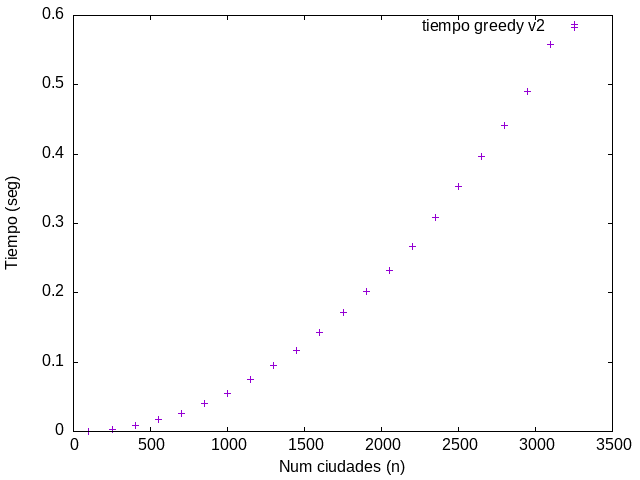
\includegraphics[width=\textwidth]{Problema4/imagenes/TSP_V2_empirica_points.png}
    \end{subfigure}
    %\hfill
    \begin{subfigure}[b]{0.45\textwidth}
        \centering
        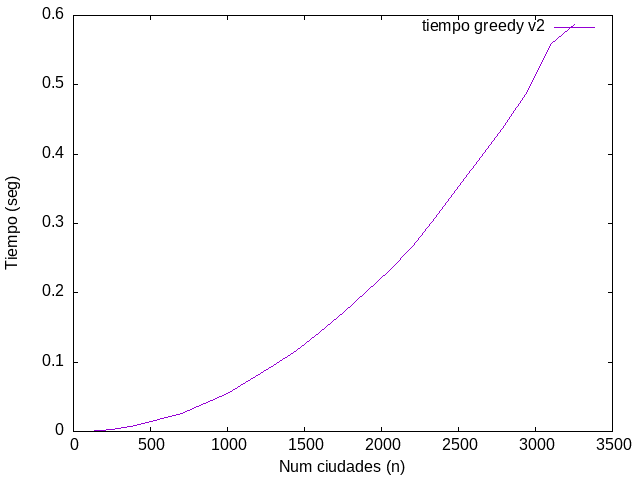
\includegraphics[width=\textwidth]{Problema4/imagenes/TSP_V2_empirica_lines.png}
    \end{subfigure}
    \caption{Eficiencia empírica de la versión 2 del TSP}
    \label{fig:p4_v2_emp}
\end{figure}

Como se puede observar en la figura (\ref{fig:p4_v2_emp}), se trata de una función claramente cuadrática, lo que coincide con el resultado demostrado en el análisis teórico.

\myparagraph{Eficiencia híbrida}
Previamente en el análisis teórico se vio que la eficiencia del algoritmo es $O(n^{2})$ y en el análisis empírico constatamos que efectivamente el algoritmo tiene complejidad cuadrática. \\

Para obtener las constantes ocultas de la ecuación de eficiencia y verificar que en efecto la función que representa la complejidad del algoritmo se trata de una función cuadrática hemos realizado una regresión cuadrática por mínimos cuadrados sobre los puntos obtenidos empíricamente con \verb|gnuplot|, es decir, con una recta de la forma $f(x) = ax^{2} + bx + c$.\\

\begin{figure}[H]
    \centering
    \begin{subfigure}[b]{0.4\textwidth}
        \centering
        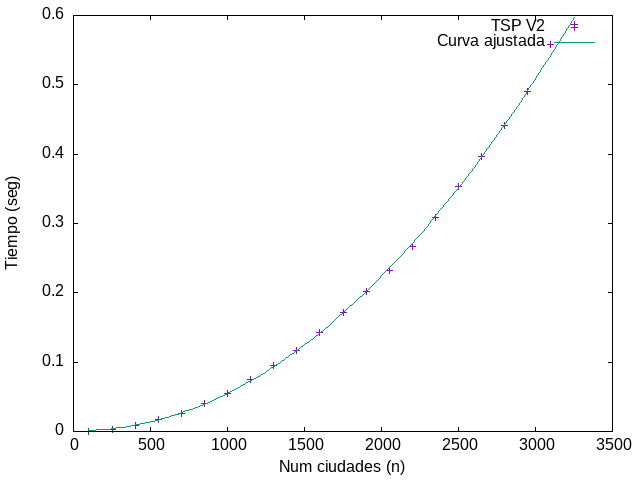
\includegraphics[width=\textwidth]{Problema4/imagenes/Salida_ajustada_v2.png}
        \caption{Gráfica ajustada de la versión 2 del TSP}
        \label{fig:p4_v2_ajuste}
    \end{subfigure}
    \hfill
    \begin{subfigure}[b]{0.5\textwidth}
        \centering
        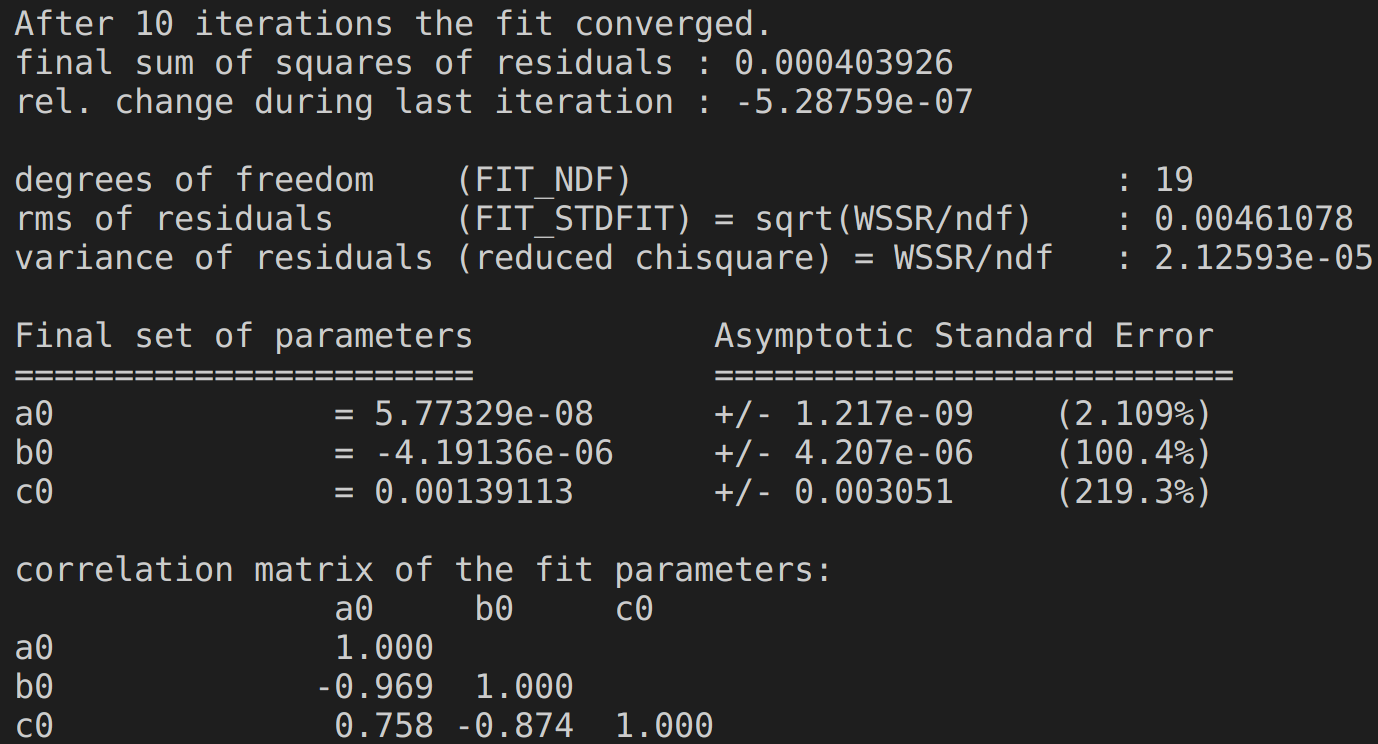
\includegraphics[width=\textwidth]{Problema4/imagenes/v2_fit_log.png}
        \caption{Regresión lineal de la versión 2 del TSP}
        \label{fig:p4_v2_fit}
    \end{subfigure}
\end{figure}

La función obtenida es:
\begin{equation*}
    f(x) = 5.77329\cdot10^{-8}x^{2} - 4.19136 \cdot10^{-5}x + 0.00139113
\end{equation*}

Como podemos observar en la figura (\ref{fig:p4_v2_fit}) la varianza residual es minúscula lo que nos indica que el ajuste realizado es el correcto, tal y como se ve en la gráfica (\ref{fig:p4_v2_ajuste}) y por tanto el algoritmo es, en efecto, $O(n^{2})$.

\subsection{Versión 3}
\subsubsection{Diseño e implementación del algoritmo voraz}
\myparagraph{Diseño}
En esta versión, aplicamos la misma heurística que en el caso
anterior pero en vez de constuir el \textit{Minimun Spanning Tree} y después listarlo en preorden, añadimos en cada paso la arista de menor coste directamente, comprobando que no se generen 
ciclos antes de tiempo y que no haya nodos de grado mayor que dos. Dadas estas recurrentes comprobaciones, este enfoque será
menos eficiente que el anterior (lo cual comprobaremos), pero 
veremos que en la mayoría de los casos las soluciones son de
mayor calidad. Veamos un ejemplo de cálculo de camino:
\begin{ejemplo}
Dadas las siguientes ciudades y sus coordenadas:
\begin{figure}[!hbt]
\centering
    \begin{subfigure}{0.3\textwidth}
    \begin{verbatim}
    13
    (0.341416,0.632643)
    (0.130035,0.90411)
    (0.334507,0.608363)
    (0.794827,0.155829)
    (0.556065,0.928201)
    (0.0531666,0.074904)
    (0.11578,0.163737)
    (0.911695,0.829456)
    (0.862248,0.792853)
    (0.0231408,0.436502)
    (0.865406,0.353367)
    (0.720413,0.040622)
    (0.11688,0.377968)
    \end{verbatim}
    \caption{Input data}
    \end{subfigure}
    \hfill
    \begin{subfigure}{0.45\textwidth}
        \centering
        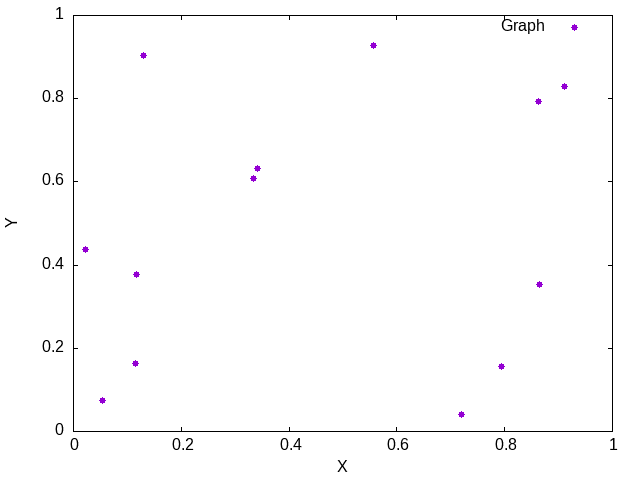
\includegraphics[width=\textwidth]{Problema4/imagenes/example_graph2.png}
        \caption{Representación gráfica}
        \label{fig:example_graph}
    \end{subfigure}
\end{figure}
\end{ejemplo}
\myparagraph{Solución}
\begin{figure}[H]
    \centering
    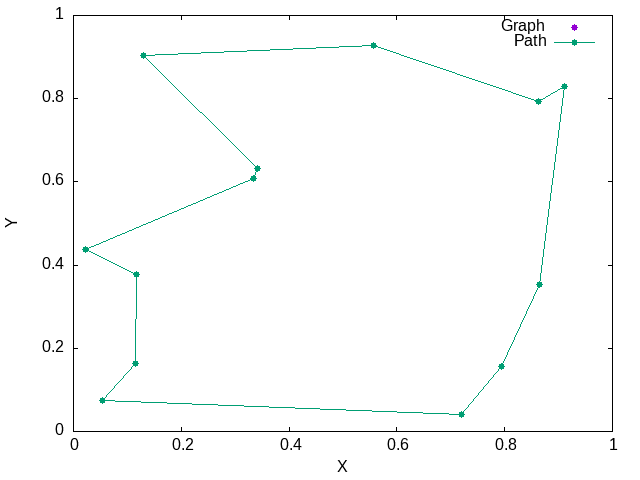
\includegraphics[scale = 0.40]{Problema4/imagenes/example_path2.png}
    \subcaption{Camino obtenido con la heurística greedy}
\end{figure} 

\myparagraph{Implementación}
Describimos cómo hemos implementado el algoritmo. La idea que hemos utilizado para controlar que no se generen ciclos es que un ciclo se genera si y solo si se unen con una arista en el grafo dos ciudades
que están en la misma componente conexa. Así, en cada paso
controlamos esta condición usando la estructura de datos del Union Find. El grado queda claramente controlado usando un vector.

La función principal del algoritmo es la siguiente:
 \lstinputlisting[language=C++, firstline=7, lastline = 7]{Problema4/codigos/greedy.cpp}
 \lstinputlisting[language=C++, firstline=63, lastline = 103]{Problema4/codigos/greedy.cpp}

 La primera parte (hata la línea 17) es clara: inicializamos
 un vector de aristas y lo ordenamos de menor a mayor en cuanto a longitudes (distancias entre ciudades: usamos el operador diferencia del tipo City). Los vectores \verb |parent| \verb |rank| \verb |degree| guardan respectivamente: un índice al nodo
 representante de la componente conexa del nodo que indexa, el
 rango del nodo que indexa (que es la profundiad aproximada
 del árbol que forma la componente conexa de la cual es representante), y el grado del nodo que indexa. El uso de \verb |rank| en este algoritmo tiene como único objetivo agilizar la búsqueda de representantes como veremos en la función \verb |union_sets|. Nótese también que la estrucutura donde almacenaremos finalmente el grafo para dar una solución es en un \verb |vector<vector<int>>tree|, en forma de lista de adyacencia. La primera función que usamos, inicializa una componente
 conexa por nodo, para posteriormente ir añadiendo aristas
y conectando componentes como corresponda hasta quedar solo con una:
 \lstinputlisting[language=C++, firstline=19, lastline = 22]{Problema4/codigos/greedy.cpp}

En el bucle tan solo insertamos en el grafo la siguiente arista
más corta controlando el grado y que no se generen ciclos, ahí entra la función \verb |union_sets| :

 \lstinputlisting[language=C++, firstline=24, lastline = 42]{Problema4/codigos/greedy.cpp}

 La función \verb|find_set| no hace más que llamarse recursivamente para
 encontrar el representante de la componente conexa de un nodo \verb|node|, consultando quién es el padre del nodo que
 se está procesando en cada paso hasta encontrar uno que
 sea su propio padre: el representante. El hecho de que
 la asignación se haga en la propia llamada en la línea 3 es un leve ajuste para ahorrar reiteradas asignaciones de los padres
 tras cada actualización: si tenemos un nodo \verb|v| a cuyo padre \verb|pv| cambiamos el padre, también estamos cambiando indirectamente el padre de \verb|v|, pero este cambio no se
 refleja en el vector \verb|parent[v]| hasta que no se pregunta por él, cuando ya es necesario.

 La función primero encuentra los padres (representantes de las
 respectivas componentes conexas) de los nodos que unimos, y
 antes de nada comprueba si están en la misma componente conexa
 (si es el caso, al unir se generarían ciclos, y entonces no lo hacemos). Ahora bien, a la hora de escoger cuál será el nuevo
 representante de la componente conexa, consultamos el \verb |rank| de ambos nodos, y enganchamos (ponemos como padre) al que 
 tenga mayor \verb |rank|, pues de lo contrario el árbol de parentesco que representa las componentes conexas resultaría
 innecesariamente profundo, lo que supondría llamadas
 extra en la función \verb|find_set|.

 Hecho esto, unimos como se espeararía añadiendo ambos
 nodos a la lista de adyacencia, para terminar una vez
 tengamos solo una componente conexa (\verb|n_sets == 1|). Es en este momento que llamamos a la función \verb|dfs| para 
 construir el camino usando el árbol de parentesco:
 \lstinputlisting[language=C++, firstline=52, lastline = 61]{Problema4/codigos/greedy.cpp}
 Esta función tan solo recorre el árbol (única componente conexa) en preorden, añadiendo
 en cada paso el nodo no visitado (cada uno los vecinos que no sea el padre del nodo que se esté procesando) a un vector de índices sobre
 el vector de ciudades que será nuestra solución (nótese que
 en este vector el índice de la primera ciudad no está repetido, es decir, que el ciclo no está cerrado: el trato del último paso se delega en la impresión de resultados 
 con la función \verb|printCycle()| ya explicada en problemas anteriores).
\subsubsection{Análisis de eficiencia}
\myparagraph{Eficiencia teórica}
Procedemos al análisis de la eficiencia teórica de la función
\verb|TSP_greedy_v3|. Primero nos econtramos con una inicalización del vector de aristas, que ya es de coste $O(n^2)$. Tras esto, notamos que la función
\verb|sort| aplicada sobre las aristas ya es de orden $O(n^4)$ en el peor caso, pues sabemos que \verb|sort| utiliza internamente el algoritmo \verb|quick_sort| y tenemos un total de $\frac{n^2-n}{2}$ aristas. Sin embargo, en la práctica,  \verb|quick_sort| se comporta como un $O(n\log(n))$, y entonces el orden
de nuestra ordenación de aristas será de $O(2n^2\log(n))$. 

Ahora bien, vemos que en el bucle \verb|while| en el que vamos
añadiendo aristas a nuestra solución (que se ejecuta del orden de $n^2$ veces en el peor caso al ser este el número de aristas) se llama a la función \verb|union_sets|. 
 \lstinputlisting[language=C++, firstline=24, lastline = 42]{Problema4/codigos/greedy.cpp}

 Esta función hace operaciones $O(1)$ y además llama a la función \verb|find_set|. Esta función sin usar la técnica de \textit{path compression} sería de orden lineal $O(n)$ puesto que en el peor de los casos debe recorrerse el 
árbol entero para dar con la componente (o padre) de un nodo. Sin embargo, dado que cada vez que le preguntamos a un nodo cual es su componente (o padre), actualizamos el padre de cada nodo entre el nodo en cuestión y su ``padre'' \textbf{comprimiendo} así el árbol de forma que no tiene eficiencia lineal en media sino de $O(log\:n)$. Solo con esto ya tenemos que la complejidad del \verb|while| será como mucho $O(n^{2}\:log\:n)$, y como se encuentra secuencial al \verb|sort| por la regla del máximo tenemos que la complejidad de la función \verb|TSP_greedy_v3| es de $O(n^{2}\:log\:n)$.

\myparagraph{Eficiencias empírica e híbrida}
Procedemos ahora a realizar un estudio de la eficiencia 
empírica del algoritmo. Los datos de tiempos desde $n=100$ hasta $n=2000$ con saltos de 100 son los siguientes:
\begin{verbatim}
100 0.006324
200 0.030369
300 0.069987
400 0.134143
500 0.211006
600 0.318191
700 0.436856
800 0.585133
900 0.756034
1000 0.952759
1100 1.15567
1200 1.40932
1300 1.6817
1400 1.63723
1500 1.38287
1600 1.57021
1700 1.79021
1800 2.01373
1900 2.30574
2000 2.55001
\end{verbatim}

\begin{figure}[H]
    \centering
    \begin{subfigure}[b]{0.45\textwidth}
        \centering
        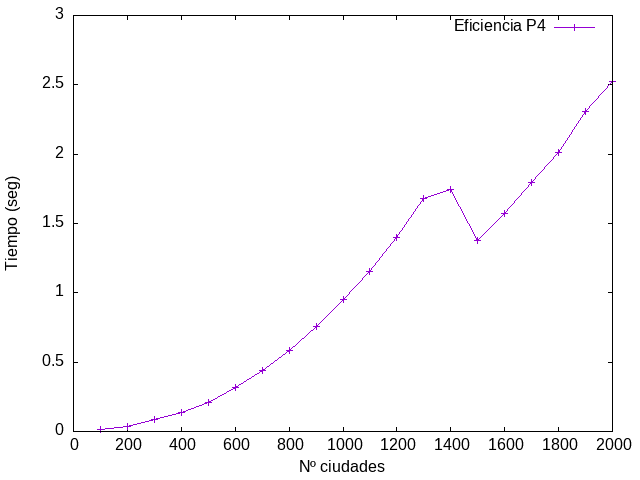
\includegraphics[width=\textwidth]{Problema4/imagenes/grafica_dani.png}
        \label{fig:tiempos_v3}
    \end{subfigure}
    %\hfill
    \begin{subfigure}[b]{0.45\textwidth}
        \centering
        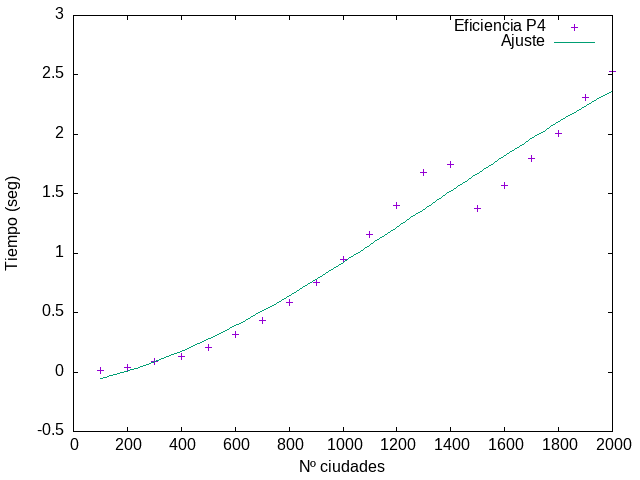
\includegraphics[width=\textwidth]{Problema4/imagenes/regresion_dani.png}
        \caption{Regresión por mínimos cuadrados}
        \label{fig:fit_v3}
    \end{subfigure}
    \caption{Eficiencias empírica e híbrida de la versión 3 del TSP}
\end{figure}

Observamos que alrededor de la zona de 1400 ciudades hay
importantes saltos en los tiempos, quizá por el hardware
sobre el que estamos ejecutando (en cuanto a reservas de memoria y demás gestiones de recursos) o por, incluso, que 
en esas instancias concretas aparezca el caso límite del \verb|quick_sort|. Para obtener las constantes ocultas que determinan la eficiencia del algoritmo hemos usado la herramienta \verb|gnuplot| y hemos obtenido los siguientes resultados:
\begin{figure}[H]
    \centering
    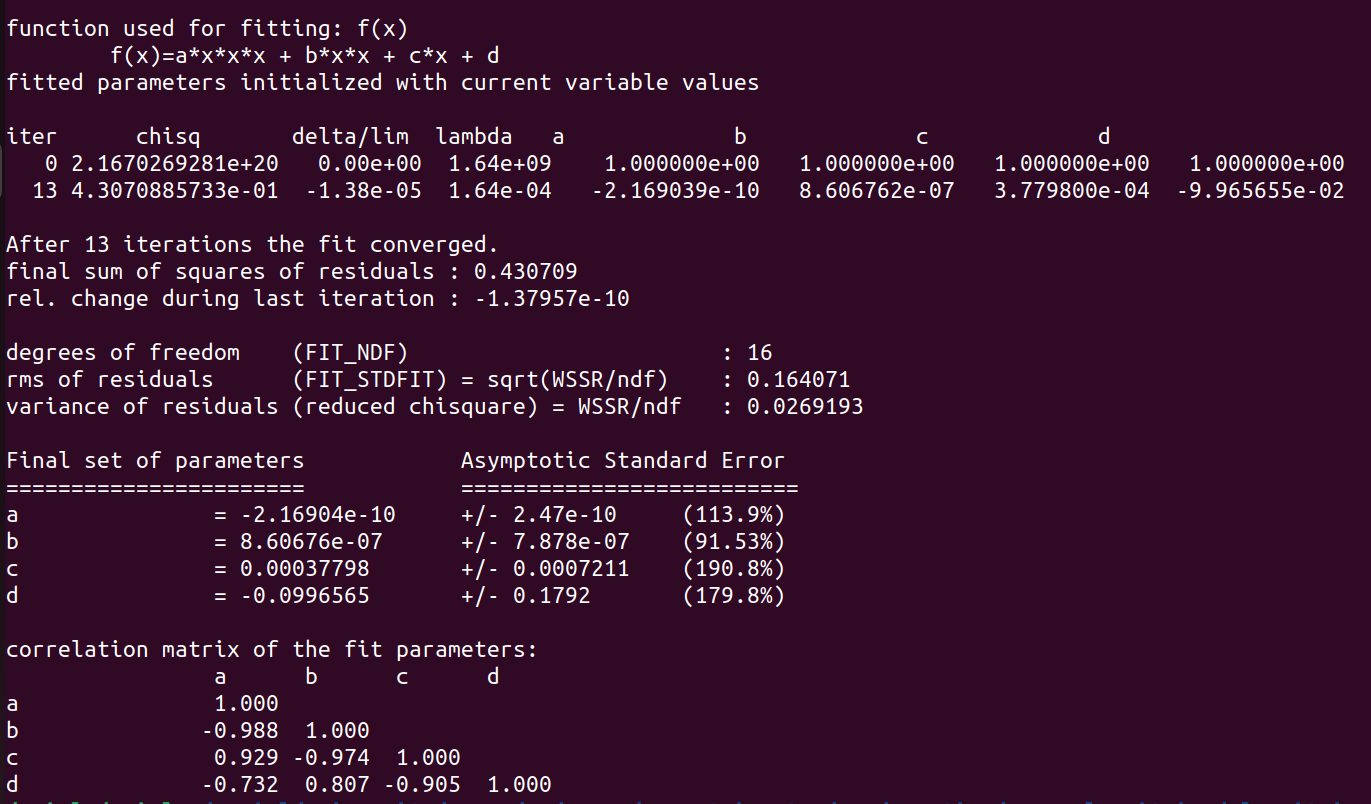
\includegraphics[width=0.7\textwidth]{Problema4/imagenes/captura_gnuplot_dani.png}
\end{figure}
Es decir, la función representada en la gráfica \ref{fig:fit_v3} que aproxima la eficiencia de nuestra función es:
\begin{equation*}
    f(x) = -2.17\cdot 10^{-10}x^3 + 8.607\cdot 10^{-7}x^2 + 
    3.78\cdot 10^{-4}x - 0.0997
\end{equation*} 

\subsection{Comparativas}
\subsubsection{Comparativa de eficiencia}

Analicemos la eficiencia de las tres versiones proporcionadas para dar una solución aproximada al problema del viajante del comercio.

\myparagraph{Eficiencia teórica}

Hemos visto previamente que las eficiencias teóricas son las de la tabla (\ref{tab:cmp_et}).
\begin{table}[hbt!]
    \centering
    \begin{tabular}{|c|c|}
        \hline
        Versión 1 & $O(n^{2})$ \\
        \hline
        Versión 2 & $O(n^{2})$ \\
        \hline
        Versión 3 & $O(n^{2}log\:n)$ \\
        \hline
    \end{tabular}
    \caption{Comparación eficiencia teórica TSP}
    \label{tab:cmp_et}
\end{table}

Tenemos pues que las versiones 1 y 2 tienen un orden de eficiencia \textbf{cuadrático} y son por tanto más rápidas que la versión 3, que es de orden $n^{2} log \: n$.

\myparagraph{Eficiencia empírica}

Para comparar la eficiencia de las tres versiones empíricamente, los tres códigos han sido ejecutados para los mismos casos de prueba, cuyos tamaños van desde $n=100$ hasta $n=1500$ cada $100$.

Los tiempos obtenidos se pueden ver en la tabla (\ref{tab:p4_time}) y las gráficas comparativas en la figura (\ref{fig:cmp_ef}).

\begin{table}[htbp]
    \centering
    \begin{tabular}{cccc} % adjust the column specifiers as needed
        \toprule
        Num ciudades (n) & Tiempo (seg) V1 & Tiempo (seg) V2 & Tiempo (seg) V3 \\
        \midrule
        100 & 0.000103 & 0.000589 & 0.002734 \\
        200 & 0.000363 & 0.002207 & 0.012647 \\
        300 & 0.000756 & 0.005126 & 0.027018 \\
        400 & 0.00161 & 0.008774 & 0.051717 \\
        500 & 0.002085 & 0.012729 & 0.081984 \\
        600 & 0.002915 & 0.018929 & 0.124607 \\
        700 & 0.00393 & 0.025662 & 0.170133 \\
        800 & 0.005131 & 0.033922 & 0.224846 \\
        900 & 0.006374 & 0.044317 & 0.289857 \\
        1000 & 0.007957 & 0.054267 & 0.364425 \\
        1100 & 0.009524 & 0.067381 & 0.443214 \\
        1200 & 0.01134 & 0.082201 & 0.536435 \\
        1300 & 0.013196 & 0.097048 & 0.641631 \\
        1400 & 0.01524 & 0.109277 & 0.743729 \\
        1500 & 0.017893 & 0.125745 & 0.858521 \\
        \bottomrule
    \end{tabular}
    \caption{Tiempos de las tres versiones del TSP}
    \label{tab:p4_time}
\end{table}

\begin{figure}[H]
    \centering
    \begin{subfigure}[b]{0.45\textwidth}
        \centering
        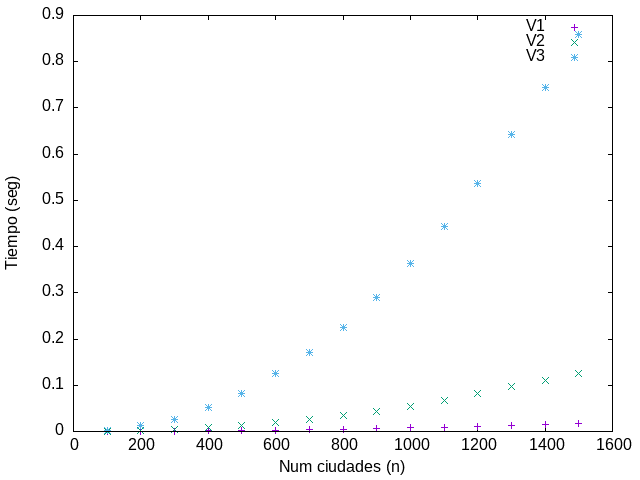
\includegraphics[width=\textwidth]{Problema4/imagenes/TSP_eficiencia_points.png}
    \end{subfigure}
    \hfill
    \begin{subfigure}[b]{0.45\textwidth}
        \centering
        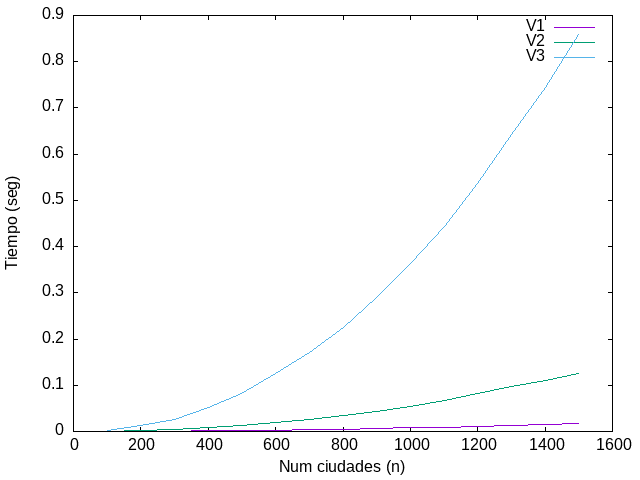
\includegraphics[width=\textwidth]{Problema4/imagenes/TSP_eficiencia_line.png}
    \end{subfigure}
    \caption{Gráficas comparativas eficiencia empírica TSP}
    \label{fig:cmp_ef}
\end{figure}

Podemos visualizar claramente que la versión 1 (closest neighbour) es la más eficiente de las tres a pesar de tener el mismo orden de eficiencia que la versión 2 (prim). Además salta a la vista que la versión 3 (kruskal) tiene un orden de eficiencia superior al de las otras dos.

\myparagraph{Eficiencia híbrida}

Finalmente presentamos una gráfica comparativa con las curvas de eficiencia de cada versión adecuadamente ajustadas en la figura (\ref{fig:cmp_hib}).

\begin{figure}
    \centering
    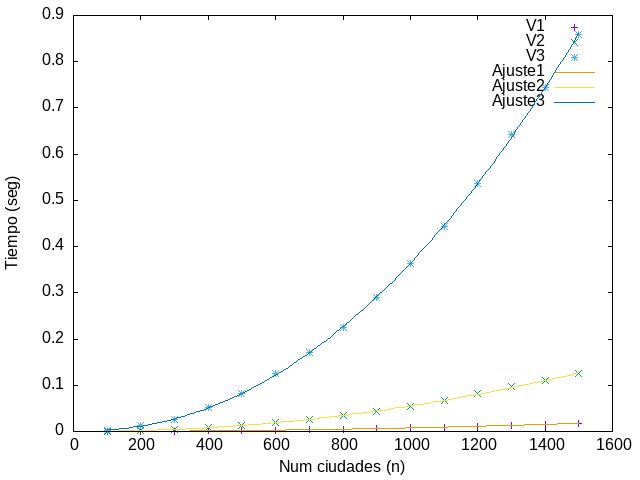
\includegraphics[width=0.75\textwidth]{Problema4/imagenes/Salida_comparativa.png}
    \caption{Comparativa eficiencia híbrida TSP}
    \label{fig:cmp_hib}
\end{figure}

Aquí confirmamos las conclusiones obtenidas en la eficiencia empírica.

\subsubsection{Comparativa de la calidad de las soluciones}

Dado que el problema del viajante de comercio es un problema NP-Díficil, no se nos es posible aportar una solución que tarde tiempo polinómico en resolver el problema. Por este motivo, todos nuestros heurísticos se limitan a dar una solución \textbf{aproximada} a la solución verdaderamente óptima del problema en cuestión.

Es por esto no solo nos interesa escoger un algoritmo eficiente, sino que también uno que nos proporcione una solución relativamente "óptima". Comparamos en la figura (\ref{fig:cmp_opt}) las soluciones aportadas por nuestro algoritmos.

\begin{figure}[H]
    \centering
    \begin{subfigure}[b]{0.45\textwidth}
        \centering
        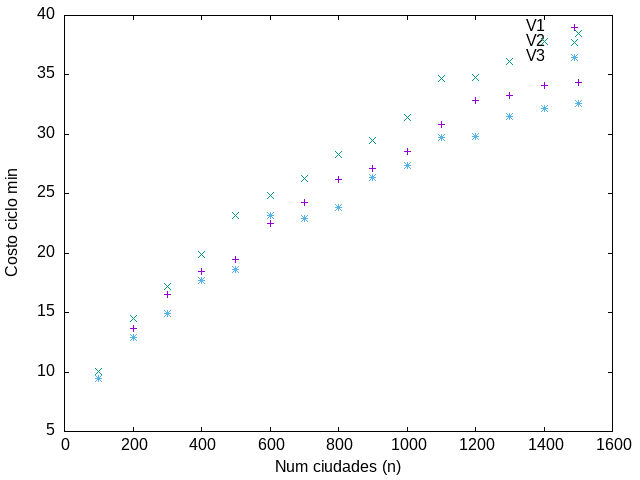
\includegraphics[width=\textwidth]{Problema4/imagenes/TSP_calidad_points.png}
    \end{subfigure}
    \hfill
    \begin{subfigure}[b]{0.45\textwidth}
        \centering
        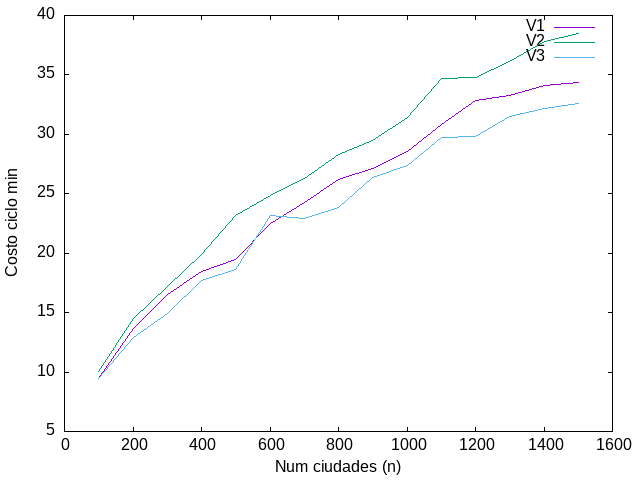
\includegraphics[width=\textwidth]{Problema4/imagenes/TSP_calidad_line.png}
    \end{subfigure}
    \caption{Gráficas comparativas eficiencia empírica TSP}
    \label{fig:cmp_opt}
\end{figure}

De ellas observamos que, las soluciones dadas por los tres algoritmos no difieren significativamente para valores pequeños de $n$. El algoritmo que proporciona una solución más óptima es la versión 3 (kruskal). Después iría la versión 1 (closest neighbour) y por último la versión 2 (prim).

\newpage
\section{Conclusiones}
A lo largo de esta práctica, hemos explorado y comprobado la efectividad y aplicabilidad del paradigma de \textbf{algoritmos voraces} en la resolución de problemas complejos de computación, complementando así los contenidos teóricos de nuestra formación.

La experiencia nos ha permitido no solo aplicar concretamente los principios teóricos, sino también observar las ventajas en términos de eficiencia que esta estrategia algorítmica ofrece. Durante el proceso, hemos enfrentado retos que destacan la importancia de la estructura de los datos de entrada y las particularidades de cada implementación en los resultados obtenidos, validando que los \textit{algoritmos voraces} son especialmente útiles para ciertos tipos de problemas que permiten un entendimiento favorable

En particular, hemos notado la manifestación de conceptos teóricos clave en la construcción de nuestros algoritmos, tales como:
\begin{itemize}
    \item La importancia de demostrar correctamente la validez y viabilidad de nuestros algoritmos voraces
    \item La observación de que las diferencias en los tiempos de ejecución al cambiar de plataforma (ya sea por hardware o software) suelen influir principalmente en una constante de proporcionalidad, pero no alteran la eficiencia comparativa entre diferentes enfoques de solución.
\end{itemize}

Esta práctica ha resultado ser una oportunidad invaluable para aplicar la teoría en un contexto práctico, enfrentando desafíos reales y desarrollando un entendimiento más profundo de los principios de diseño de algoritmos. Consideramos que esta experiencia ha sido exitosa, enriqueciendo nuestra preparación para enfrentar futuras problemáticas en nuestro camino académico y profesional, y proporcionando herramientas y perspectivas esenciales para identificar casos en los cuales la estrategia de \textbf{algoritmos voraces} es adecuada y cómo implementarla efectivamente.

\end{document}
